\chapter{Curvature of space}
\pagebreak[4]

\section{p82 - Exercise}
\begin{tcolorbox}
Explain why the surfaces of an ordinary cylinder and an ordinary cone are to be regarded as "flat" in the sense of our definition.
\end{tcolorbox}
The reason is because those surfaces can be "unwrapped" like the figure below shows. 
\begin{figure}[h]
%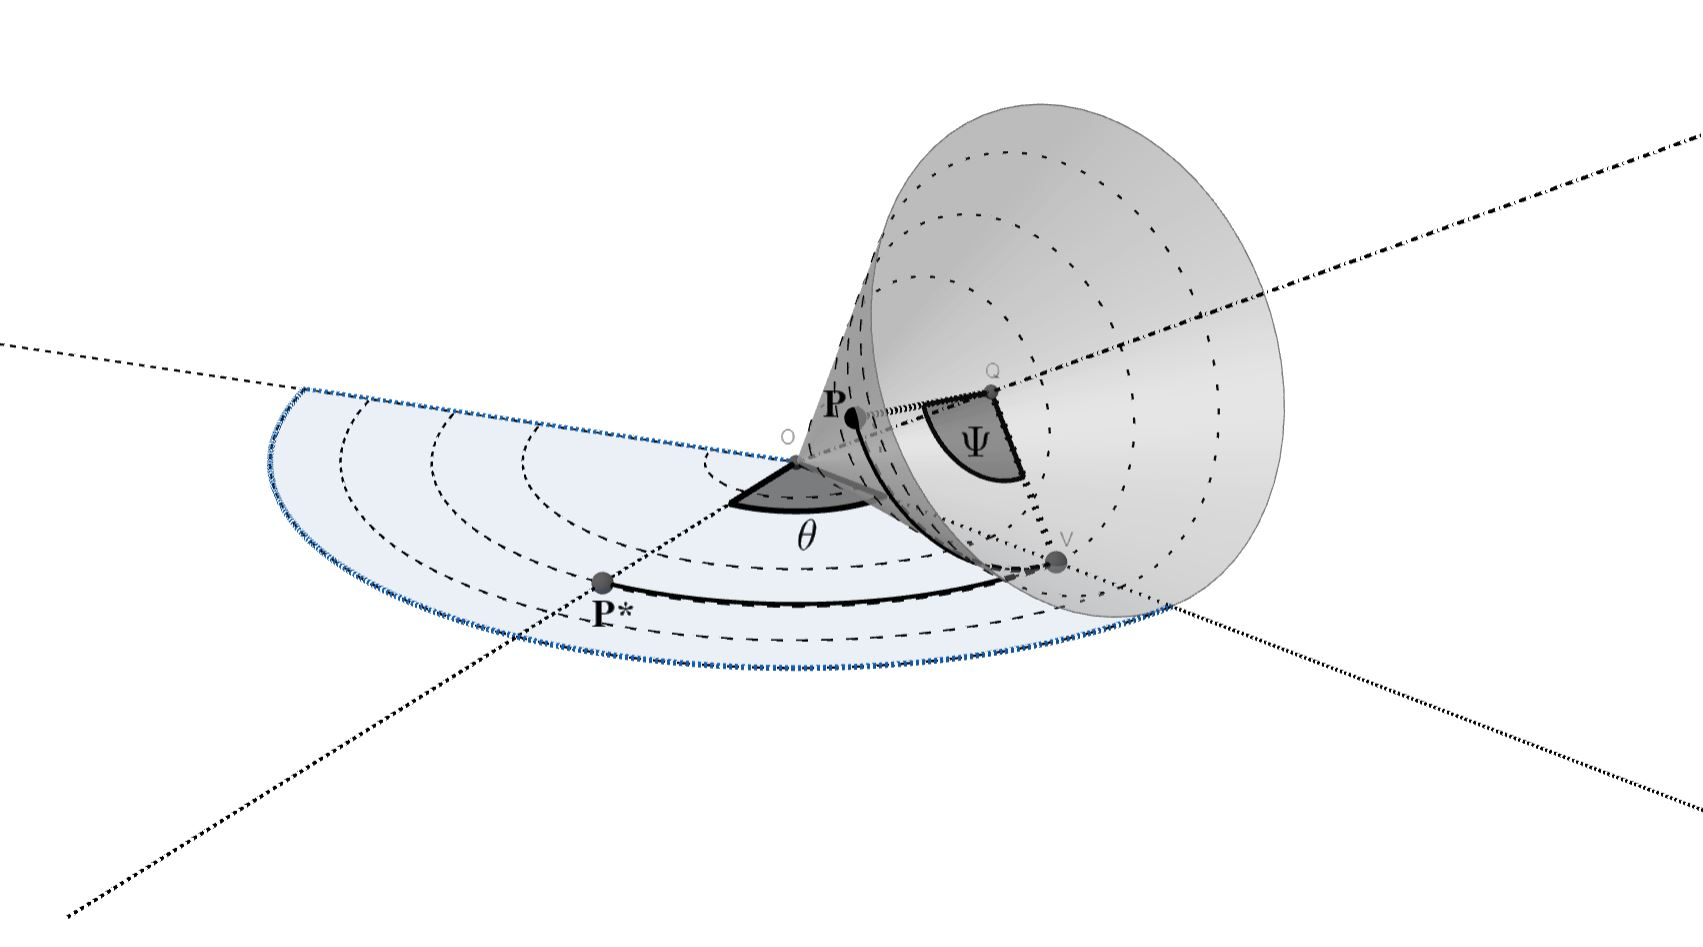
\includegraphics[scale=.5]{Conemapping.jpg}
%\tdplotsetmaincoords{0}{10};
\pgfplotsset{every axis/.append style={
		view={-30}{-30*1},
		%view={-90}{-30*0},
		scale=1.5,
		axis lines=center,
		axis on top,
		%xlabel={$y$},
		%ylabel={$x$},
		%zlabel={$z$},
               axis x line=middle,    % put the x axis in the middle
               axis y line=middle,    % put the y axis in the middle
                axis z line=middle,    % put the z axis in the middle
               %axis line style={-stealth}, % arrows on the axis
               axis line style={draw=none}
            }}
            


            
\begin{tikzpicture}[angle/.style={black,thick}]
\tikzmath{\r=1.5;\h=5;\q=asin((\r/\h)); \p=-\q*1 ; \k= \r/\h;};
\q, \h,\p, \k;
    \pgfplotsset{ticks=none};
    \pgfplotsset{compat=1.12};
\begin{axis}
		[
		axis equal=true,
		zmin=-\h*0,
		zmax=\r*1.2,
		]
		%draw the cylinder whiwh is tilted so that it 'rolls' on the x-y plane and oriented along the y-axis
		\addplot3 [surf,dashed,very thin,	mesh/interior colormap=
		{bw}{color=(gray!10) color=(gray!5)},
		colormap= {bw}{color=(black!10) color=(white!10)},
		domain=115:115+180,
		y domain=0:\h,
		samples=40,
		samples y=10,
		z buffer=sort,]
		({\y*cos(\p)+1*\y*tan(\q)*sin(x)*sin(\p)},{1*y*tan(\q)*cos(x)},{-\y*sin(\p)+1*\y*tan(\q)*sin(x)*cos(\p)});
		
		
		%draw the cylinder whiwh is tilted so that it 'rolls' on the x-y plane and oriented along the y-axis
		\addplot3 [surf,	dashed,thick,	mesh/interior colormap=
		{bw}{color=(gray!1) color=(gray!5)},
		colormap= {bw}{color=(black!1) color=(white!1)},
		domain=-65:115,
		y domain=0:\h,
		samples=40,
		samples y=10,
		z buffer=sort,]
		({\y*cos(\p)+1*\y*tan(\q)*sin(x)*sin(\p)},{1*y*tan(\q)*cos(x)},{-\y*sin(\p)+1*\y*tan(\q)*sin(x)*cos(\p)});
	
		%add a base circle to emphasize the cone shape
		\addplot3 [black,thick,dashed,samples=40,	samples y=0,	domain=0.0:360,]({\h*cos(\p)+1*\h*tan(\q)*sin(x)*sin(\p)},{1*\h*tan(\q)*cos(x)},{-\h*sin(\p)+1*\h*tan(\q)*sin(x)*cos(\p)});
		% add an arcsegment on the base
		\addplot3 [decoration={markings, mark = at position 0.5 with {\arrow[scale = 1.5]{latex}}},postaction ={decorate},black,thick,samples=40,	samples y=0,	domain=60:-90,]({\h*cos(\p)+1*\h*tan(\q)*sin(x)*sin(\p)},{1*\h*tan(\q)*cos(x)},{-\h*sin(\p)+1*\h*tan(\q)*sin(x)*cos(\p)});%node[midway,right] {$\Psi$};;
		% add an arcsegment at 2/3 pf the cone
		\addplot3 [decoration={markings, mark = at position 0.5 with {\arrow[scale = 1.5]{latex}}},postaction ={decorate},black,thick,samples=40,	samples y=0,	domain=60.0:-90,]({2*\h/3*cos(\p)+2*\h/3*tan(\q)*sin(x)*sin(\p)},{2*\h/3*tan(\q)*cos(x)},{-2*\h/3*sin(\p)+2*\h/3*tan(\q)*sin(x)*cos(\p)});%node[midway,right] {$x^1$};
		
		
		% labels of arcsegments on the cone
		 \coordinate (F) at ({2*\h/3*cos(\p)+2*\h/3*tan(\q)*sin(20)*sin(\p)},{2*\h/3*tan(\q)*cos(20)},{-2*\h/3*sin(\p)+2*\h/3*tan(\q)*sin(20)*cos(\p)});
 		\draw[](F) node[{anchor=north west}] {$\theta$};
 		\coordinate (F2) at ({\h*cos(\p)+\h*tan(\q)*sin(20)*sin(\p)},{\h*tan(\q)*cos(20)},{-\h*sin(\p)+\h*tan(\q)*sin(20)*cos(\p)});
 		\draw[](F2) node[{anchor=north west}] {$\theta$};
 		
		%relevant points
		\coordinate (O) at ({ 0},{0},{0});%origin
		\coordinate (P) at ({ \h*1},{\h*0},{0});%point  P on the cone 
		\coordinate (C) at ({1.2* \h*cos(\p)},{\h*0},{1.2*\h*sin(-\p)});
		\coordinate (A) at ({1.* \h*cos(\p)},{\h*0},{1.*\h*sin(-\p)});
		\coordinate (Q) at ({1.* \h/cos(\p)},{\h*0},{0.*\h*sin(-\p)});

		%\node[tdplot_main_coords,{anchor=south west},red] at (P){$o$};
		%\draw[dashed,line width = 0.25mm] (O) --(P) ;%node[midway,right] {$x^1$};
		\draw[dashdotted,- latex,line width = 0.25mm] (O) --(C) ;%node[midway,right] {$x^1$};
		%\draw[dashdotted,line width = 0.25mm] (Q) --(A) ;%node[midway,right] {$x^1$};
		%draw points on cone
		\coordinate (W) at ({ \h/cos(\p)},{\h*0},{0.*\h*sin(-\p)});
		\coordinate (N) at ({1.2 *\h},{\h*0},{0.*\h*sin(-\p)});
		\coordinate (R) at ({2/3* \h/cos(\p)},{\h*0},{0.*\h*sin(-\p)});
		\coordinate (S) at ({2*\h/3*cos(\p)+2*\h/3*tan(\q)*sin(60)*sin(\p)},{2*\h/3*tan(\q)*cos(60)},{-2*\h/3*sin(\p)+2*\h/3*tan(\q)*sin(60)*cos(\p)});
		\coordinate (T) at ({2*\h/3*cos(\p)+0*\h/3*tan(\q)*sin(60)*sin(\p)},{0},{-2*\h/3*sin(\p)+0*\h/3*tan(\q)*sin(60)*cos(\p)});
		\draw[fill=black](A) circle(1.5pt);%node[{anchor=north west}] {$A$};
		\draw[fill=black](Q) circle(1.5pt);%node[{anchor=north west}]{$A$};;
		\coordinate (Y) at ({\h*cos(\p)+\h*tan(\q)*sin(60)*sin(\p)},{\h*tan(\q)*cos(60)},{-\h*sin(\p)+\h*tan(\q)*sin(60)*cos(\p)});
		\draw[fill=black](Y) circle(1.5pt)node[{anchor=south east}] {$R$};
		\draw[fill=black](W) circle(1.5pt);%node[{anchor=north west}] {$O$};;
		\draw[fill=black](R) circle(1.5pt);%node[{anchor=north west}]{$V$};;
		\draw[fill=black](S) circle(1.5pt)node[{anchor=south east}] {$P$};
		\draw[fill=black](T) circle(1.5pt)node[{anchor=south west}] {$o$};
		\draw[dashdotted,- latex,line width = 0.25mm] (O) --(N) ;%node[midway,right] {$x^1$};
		\draw[dashdotted,line width = 0.25mm] (T) --(R) ;%node[midway,right] {$x^1$};
		\draw[dashdotted,line width = 0.25mm] (T) --(S) ;%node[midway,right] {$x^1$};
		
		\draw[dashdotted,line width = 0.25mm] (Y) --(A) ;%node[midway,right] {$x^1$};
		\draw[dashdotted,line width = 0.25mm] (Y) --(S) ;%node[midway,right] {$x^1$};
		\draw[dashdotted,line width = 0.25mm] (W) --(A) ;%node[midway,right] {$x^1$};


		
		%projection onthe xy-plane
		%arcsegments of points P and R
		\begin{scope}
		\addplot3 [decoration={markings, mark = at position 0.5 with {\arrow[scale = 1.5]{latex}}},postaction ={decorate},samples=40,black,thick,samples=40,	samples y=0,	domain=0:150,]
			({2/3*\h/cos(\q)*cos(x*sin(\q))},{2/3*\h/cos(\q)*sin(x*sin(\q))},{0});%node[midway,right] {$theta$};
		\addplot3 [decoration={markings, mark = at position 0.5 with {\arrow[scale = 1.5]{latex}}},postaction ={decorate},samples=40,black,thick,samples=40,	samples y=0,domain=0:150,]
			({\h/cos(\q)*cos(x*sin(\q))},{\h/cos(\q)*sin(x*sin(\q))},{0});%node[midway,right] {$x^1$};
		\end{scope}
		%projections  R*, P* of points R,P
		\coordinate (U) at ({2/3*\h/cos(\q)*cos(150*sin(\q))},{2/3*\h/cos(\q)*sin(150*sin(\q))},{0});
		\coordinate (V) at ({\h/cos(\q)*cos(150*sin(\q))},{\h/cos(\q)*sin(150*sin(\q))},{0});
		

		\draw[dashdotted,line width = 0.25mm] (O) --(U) ;%node[midway,right] {$x^1$};
		\draw[dashdotted,line width = 0.25mm] (O) --(V) ;%node[midway,right] {$x^1$};
		
		%dots and labels of P* and R*
 		
 		\draw[fill=black](U) circle(1.5pt)node[{anchor=north east}] {$P^{*}$};
		\draw[fill=black](V) circle(1.5pt)node[{anchor=north east}] {$R^{*}$};
 		%add labels of angles at a right place
 		 \coordinate (G) at({2/3*\h/cos(\q)*cos(90*sin(\q))},{2/3*\h/cos(\q)*sin(90*sin(\q))},{0});
 		\draw[](G) node[{anchor=south east}] {$\phi$};
 		 \coordinate (M)  at({\h/cos(\q)*cos(90*sin(\q))},{\h/cos(\q)*sin(90*sin(\q))},{0});
 		\draw[](M) node[{anchor=north west}] {$\phi$};
\end{axis}
\end{tikzpicture}\\
\caption{Unwrapping of a cone}
\end{figure}\\
For the cone, we can for each point $\ P $ on the cone, lying on a distance $\ h $ from the apex and making an angle $\Psi $,  associate on a plane,  a  point $ P^* $ lying at the same  distance $ h $ from the apex, taken as origin for the coordinate system, and making an angle $\theta =  k\Psi $ with $ k $ a constant depending on the shape of the cone. This pair of coordinates are polar coordinates with $ r \in (-\infty, + \infty)$ and $\theta \in [0, 2k\pi)$. 
The same reasoning can be applied to a cylinder which is a cone with the apex at $\infty$. In that case the coordinate system becomes a Cartesian coordinate system. \\
As a continuous mapping exist from polar to orthogonal Cartesian coordinates both  coordinate system can be written under the required form (3.101) and so can be called "flat".

$$\blacklozenge$$
\newpage

\section{p83 - Exercise}
\begin{tcolorbox}
What are the values of $R^s_{.rmn}$ in an Euclidean plane, the coordinates being rectangular Cartesians? Deduce the values of the components of this tensor for polar coordinates from its tensor character, or else by direct calculation.
\end{tcolorbox}
See 2.64 page 139 (exercise 18).
$$\blacklozenge$$
\newpage

\section{p86 - Exercise}
\begin{tcolorbox}
Show that in a $V_2$ all the components of the covariant curvature tensor either vanish or are expressible in terms of $R_{1212}$.
\end{tcolorbox}
We have (3.115) and (3.116)
\begin{align}
\left \{ \begin{array}{l}
\ R_{rsmn} =  - R_{srmn}\\
\ R_{rsmn} =  - R_{rsnm}\\
\ R_{rsmn} =   R_{mnrs}\\
\ R_{rsmn} + R_{rmns}+R_{rnsm}=0
\end{array} \right.
\end{align}
It is clear from the two first identities that  in pairs $(rs)$ and $(mn)$ both indices have to be different when the tensor is not $0$. So we only have to consider $R_{1212}$,  $R_{1221}$, $R_{2112}$ and $R_{2121}$.\\
The two first  identities gives us:
\begin{align}
 R_{1221}= -R_{1212}\\
 R_{2112}= -R_{1212}\\
 R_{2121}= -R_{2112} = R_{1212}
\end{align}
The third identity does give us any additional information.
The fourth identity gives us only trivial statements:
\begin{align}
 R_{1212} + \underbrace{R_{1122}}_{=0}+\underbrace{R_{1221}}_{=- R_{1212} } = 0\\
 \underbrace{R_{1221}}_{=- R_{1212}} + R_{1212}+\underbrace{R_{1122}}_{=0 } = 0\\
 \underbrace{R_{2112}}_{=- R_{1212}} + \underbrace{R_{2121}}_{=R_{1212}}+\underbrace{R_{2211}}_{=0} = 0\\
 \underbrace{R_{2121}}_{= R_{1212}} + \underbrace{R_{2211}}_{=0}+\underbrace{R_{2112}}_{= -R_{1212}} = 0
\end{align}
$\textbf{Conclusion:}$\\
We get the identities (2), (3) and (4) in function of $R_{1212}$ and all vanish if $R_{1212} = 0$
$$\blacklozenge$$
\newpage

\section{p86-87 - clarification}
\begin{tcolorbox}
\textit{The number of independent components of the covariant curvature tensor in a space of N dimensions is} $$\frac{1}{12}N^2\left(N^2-1\right)$$
\end{tcolorbox}
We have (3.115) and (3.116)
\begin{align}
\left \{ \begin{array}{l}
R_{rsmn} =  - R_{srmn}\\
R_{rsmn} =  - R_{rsnm}\\
R_{rsmn} =   R_{mnrs}\\
R_{rsmn} + R_{rmns}+R_{rnsm}=0
\end{array}\right.
\end{align}
It is clear from the two first identities that  in the tuple $(rs)$ and $(mn)$ both indices have to be different when the component is not $0$. So we only have to consider the component with the pair of tuples $(r,s)$ and $m,n)$ with $r \neq s$ and $m \neq n$.
For the tuple $(r,s)$ we have $N$ possibilities to draw an index for $r$ but for $s$ only $N-1$ indices remain as $r \neq s$. So for the tuple $(r,s)$ we get $N(N-1)$ possibilities. But note by the first identity $R_{rsmn} =  - R_{srmn}$ that we only have to consider the half of this quantity as once we have chosen a tuple $(r,s)$ we also know  the component for the tuple $(s,r)$. So the total number of possibilities we have for  $(r,s)$ is $M = \half N(N-1)$. The same yields for the tuple $(mn)$. So, we get in total $M^2$ possibilities according to the two first identities.\\
The third identity $R_{rsmn} =   R_{mnrs}$ puts an extra constraint on the number of possibilities as we have to subtract from $M^2$ the number of possibilities covered by this third identity. Note that, once we have chosen a tuple $(rs)$ we have to exclude the tuple $(m,n) =  (r,s)$ as the identity $R_{rsrs} =   R_{rsrs}$ becomes trivial.. So for the first tuple we have $M$ possibilities, but once chosen, only $M-1$ remain for the second tuple. So we get $M(M-1)$ possibilities. But, again we only have to take half of these possibilities as the identities $R_{rsmn} =   R_{mnrs}$ and $ R_{mnrs} = R_{rsmn}$ are equivalent.\\
So the total number of possibilities reduces to $$ M^2 - \half M(M-1) \quad \text{with} \quad M=\half N(N-1) $$
What about the fourth identity $$R_{rsmn} + R_{rmns}+R_{rnsm}=0$$
First we note that this identity implies that all indices are different as it becomes trivial in the other cases. This is a consequence of the first 3 identities. Indeed, we know already that
\begin{align}
\left \{ \begin{array}{l}
\ r \neq s\\
\ m \neq n\\
\ (r,s) \neq (m,n)\\
\end{array} \right.
\end{align}
Let's consider the following cases
\begin{align}
\left \{ \begin{array}{llll}
\ r = m&\rightarrow m\neq s \  m\neq n \ r\neq n&\rightarrow & R_{rsrn} + \underbrace{R_{rrns}}_{=0}+\underbrace{R_{rnsr}}_{= -R_{rnrs}= -R_{rsrn}}=0\\
\ r = n&\rightarrow n\neq s \  m\neq n \ r\neq s&\rightarrow & R_{rsmr} + \underbrace{R_{rmrs}}_{= -R_{mrrs}= -R_{rsmr}}+\underbrace{R_{rrsm}}_{=0}=0\\
\ s = m&\rightarrow m\neq r \  n\neq s \ r\neq s&\rightarrow & R_{rssn} + \underbrace{R_{rsns}}_{= -R_{rssn}}+\underbrace{R_{rnss}}_{=0}=0\\
\ s = n&\rightarrow r\neq s \  m\neq s \ m\neq n&\rightarrow & R_{rsms} + \underbrace{R_{rmss}}_{=0}+\underbrace{R_{rssm}}_{= -R_{rsms}}=0
\end{array} \right.
\end{align}
So indeed, once two indices are equal, the fourth identity becomes trivial and does not put extra constraints to the number of possibilities. For the tuple $(r,s,m,n)$ we have $N$ possibilities to draw an index for $r$, for $s$ only $N-1$, for $m$ only $N-2$ and for $n$ only $N-3$ indices remain as $r \neq s\neq m\neq n$. The maximum number of constraint generated by the fourth identity is thus $$N(N-1)(N-2)(N-3)$$
But here again double counts occur. Indeed the fourth identity is true for the $6$ tuples $$(rsmn),(rmsn) ,(rmns),(rsnm),(rnsm),(rnms)$$ as first entry    in the identity. The same reasoning is valid for the tuples $(n...), \ (s...) \ (m...) $. \\So in total we get $6\times4 = 24$ equivalent identities and the number of constraints generated by the fourth identity reduces to  $$\frac{1}{24}N(N-1)(N-2)(N-3)$$
Note that this number of constraints vanish for $N \leq 3$.\\
Putting it all together the number of independent components of $R_{rsmn}$ becomes
\begin{align}
\mho &= M^2 - \half M(M-1)-\frac{1}{24}N(N-1)(N-2)(N-3)\\
&= \half M(M+1)-\frac{1}{24}N(N-1)(N-2)(N-3)\\
&= \frac{1}{8} N(N-1) \left(N(N-1)+2\right)-\frac{1}{24}N(N-1)(N-2)(N-3)\\
&= \frac{N}{24} \left( 3N^2-6N^2+9N-6-N^3+3N^2+3N^2-9N-2N+6 \right)\\
&= \frac{1}{12}N^2 \left( N^2-1\right)
\end{align}
$$\blacklozenge$$
\newpage

\section{p87 - Exercise}
\begin{tcolorbox}
Using the fact that the absolute derivative of the fundamental tensor vanishes, prove that 3.107 may be written $$ \frac{\delta^2 T_r}{\delta u \delta v} - \frac{\delta^2 T_r}{\delta v \delta u} = R_{rpmn}T^p\partial_u x^m \partial_v x^n $$
\end{tcolorbox}
By 2.519 and 2.619 we have
\begin{align}
\fdv{T_r}{u} &= \fdv{(a_{rk}T^k)}{u} 
 = \underbrace{\fdv{(a_{rk})}{u}}_{=0}T^k+a_{rk}\fdv{(T^k)}{u}\\
 &= a_{rk}T^k_{|n} \partial_u x^n\\
 \Rightarrow\quad \frac{\delta^2 T_r}{\delta u \delta v} &= \frac{\delta (a_{rk}T^k_{|n} \partial_u x^n)}{\delta v}\\
  & = \underbrace{\frac{\delta (a_{rk})}{\delta v}}_{=0}T^k_{|n} \partial_u x^n+a_{rk}\frac{\delta (T^k_{|n} )}{\delta v}\partial_u x^n+a_{rk}T^k_{|n} \delta \frac{(\partial_u x^n)}{\delta v}\\
   &= a_{rk}\underbrace{\frac{\delta (T^k_{|n} )}{\delta v}}_{=T^k_{|nm}\partial_v x^m} \partial_u x^n+a_{rk}T^k_{|n} \underbrace{\delta \frac{(\partial_u x^n)}{\delta v}}_{=\left(\partial_u x^n \right)_{|m}\partial_v x^m}\\
   &= a_{rk}T^k_{|nm}\partial_v x^m \partial_u x^n+a_{rk}T^k_{|n} \underbrace{\left(\partial_u x^n \right)_{|m}}_{ = \partial_m \left(\partial_u x^n \right) + \Gamma^n_{pm}\partial_u x^p}\partial_v x^m\\
   &= a_{rk}T^k_{|nm}\partial_v x^m \partial_u x^n+a_{rk}T^k_{|n} \left( \underbrace{\partial_m \left(\partial_u x^n \right)}_{=\partial_u \left( \delta_m^n \right)=0} + \Gamma^n_{pm}\partial_u x^p \right)\partial_v x^m\\
   &= a_{rk}T^k_{|nm}\partial_v x^m \partial_u x^n+a_{rk}T^k_{|n} \Gamma^n_{pm}\partial_u x^p \partial_v x^m
\end{align}
Hence we have 
\begin{align}
\frac{\delta^2 T_r}{\delta v \delta u} &=a_{rk}T^k_{|nm}\partial_u x^m \partial_v x^n+a_{rk}T^k_{|n} \Gamma^n_{pm}\partial_v x^p \partial_u x^m\\
&=a_{rk}T^k_{|mn}\partial_u x^n \partial_v x^m+a_{rk}T^k_{|n} \Gamma^n_{mp}\partial_v x^m \partial_u x^p\\
\Rightarrow\quad \frac{\delta^2 T_r}{\delta u \delta v} - \frac{\delta^2 T_r}{\delta v \delta u} &= a_{rk}T^k_{|nm}\partial_v x^m \partial_u x^n - a_{rk}T^k_{|mn}\partial_u x^n \partial_v x^m\\
&= \left(a_{rk}T^k_{|nm} - a_{rk}T^k_{|mn}\right)\partial_u x^n \partial_v x^m\\
&= \left(\underbrace{T_{r|nm} - T_{r|mn}}_{= -R_{rpmn}T^p}\right)\partial_u x^n \partial_v x^m\\
&= -\underbrace{R_{rpmn}}_{=-R_{rpnm}} T^p\partial_u x^n \partial_v x^m = 
R_{rpmn} T^p\partial_u x^m \partial_v x^n
\end{align}
$$\blacklozenge$$
\newpage

\section{p91 - Exercise}
\begin{tcolorbox}
Would the study of geodesic deviation enable us to distinguish between a plane and a right circular cylinder?
\end{tcolorbox}
For geodesic lines we have
\begin{align}
\dv[2]{x^r}{u} + \Gamma^r_{mn}\dv{x^m}{u}\dv{x^n}{u} = 0\\
\end{align}
with the fundamental tensor for a cylinder (see exercise page 27)
\begin{align} 
(a_{mn}) = \begin{pmatrix}
 1& 0 \\
0 & r^2 \\
\end{pmatrix}
\end{align}
As no element of this tensor is a function of the coordinates, it is clear that all Christoffel symbols vanish and the geodesic curve are solutions of the simple system of $2^{nd}$ order differential equations
\begin{align}
\dv[2]{x^r}{u}  = 0
\end{align}
Hence
\begin{align}
x^r  &= \kappa u + \mu\\
\text{or}\quad x^r &= \kappa^r u
\end{align}
by choosing the origin of the coordinates system with the initial condition position of the point.
Choosing polar coordinates $\phi, z$ as coordinates, the distance one walks when following a geodesic is given by
\begin{align}
 s= \int_{u_0}^{u_1}\sqrt{(r^2(d\phi)^2 + (dz)^2)}
\end{align}
and if we take $u=\phi$ as independent a parameter, by (6) we get 
\begin{align}
 s-s_0 &= \int_{\psi_0}^{\psi_1}\sqrt{(r^2 + \kappa^2)}d\psi \equiv g(\psi - \psi_0)\\
 \text{or}\quad s&= \int_{\psi_0}^{\psi_1}\sqrt{(r^2 + \kappa^2)}d\psi \equiv g\psi
\end{align}
by introducing transformed coordinates $s^{'}= s-s_0$ and $\psi^{'} =\psi - \psi_0$.\\
and thus we get 
\begin{align}
 z = m s^{'}
\end{align}
\begin{figure}[H]
%\centering
\begin{minipage}[t]{.4\textwidth}
%\centering
\vspace{0pt}
%\includegraphics[scale=.5]{p85_ex1.png}
\tdplotsetmaincoords{0}{10};
\pgfplotsset{every axis/.append style={
		view={-10*1}{-30*1},
		%view={-90}{-30*0},
		scale=2.5,
		%axis lines=center,
		axis on top,
		xlabel={$y$},
		ylabel={$x$},
		zlabel={$z$},
               axis x line=middle,    % put the x axis in the middle
               axis y line=middle,    % put the y axis in the middle
                axis z line=middle,    % put the z axis in the middle
               axis line style={-stealth}, % arrows on the axis
            }}
\begin{tikzpicture}

  \def\r{0.5};
    \def\H{10};
    \pgfplotsset{ticks=none};
    \pgfplotsset{compat=1.12};

    	
\begin{axis}
		[
		xmin=-1.5,
		xmax=1.5,
		ymin=-1.5,
		ymax=1.5,
		zmin=0.0,
		zmax=10.0,
		]
		%draw the cylinder
		\addplot3 [surf,	dashed,thick,domain=0:10,	mesh/interior colormap=
		{bw}{color=(gray!10) color=(gray!50)},
		colormap= {bw}{color=(white!10) color=(white!10)},
		y domain=0:1*pi,samples=10,
		samples y=40,z buffer=sort,]
		({\r*cos(deg(y))},{\r*sin(deg(y))},{x});
						%draw the curves
				%base cylinder
		
		\addplot3 +[no markers,dotted,thick, black,samples=51,	samples y=0,	domain=-pi/2+0.16666667:pi/2+0.16666667,variable=\t]
		({0.5*sin(deg(\t))},{0.5*cos(deg(\t))},{0 });
		\addplot3 +[no markers,dotted,gray,thick, black,samples=51,	samples y=0,	domain=0:2*pi,variable=\t]
		({0.5*sin(deg(\t))},{0.5*cos(deg(\t))},{10 });		
		\addplot3 +[no markers,dotted,gray,thick, black,samples=51,	samples y=0,	domain=-pi/2+0.16666667:pi/2+0.16666667,variable=\t]
		({0.5*sin(deg(\t))},{0.5*cos(deg(\t))},{5 });	
		
		
				%curve1
		\addplot3 [ultra thick, black,samples=51,	samples y=0,	domain=0:pi/2+0.16666667,variable=\t]
		({0.5*sin(deg(\t))},{0.5*cos(deg(\t))},{\t });
		
		\addplot3 [thick, dashed,thick,black,samples=51,	samples y=0,	domain=pi/2+0.16666667:3*pi/2+0.17776667,variable=\t]
		({0.5*sin(deg(\t))},{0.5*cos(deg(\t))},{\t });
		
			\addplot3 [ultra thick, black,samples=51,	samples y=0,	domain=3*pi/2+0.17776667:2*pi,variable=\t]	
		({0.5*sin(deg(\t))},{0.5*cos(deg(\t))},{\t });
		

		
		%curve2
			\addplot3 [ultra thick, black,samples=51,	samples y=0,	domain=0:pi/2+0.16666667,variable=\t]
		({0.5*sin(deg(\t))},{0.5*cos(deg(\t))},{\t*1.5 });
		
		\addplot3 [dashed,thick,black, samples=51,	samples y=0,	domain=pi/2+0.16666667:3*pi/2+0.17776667,variable=\t]	
		({0.5*sin(deg(\t))},{0.5*cos(deg(\t))},{\t*1.5});
		
		\addplot3 [ultra thick, black,samples=51,	samples y=0,	domain=3*pi/2+0.17776667:2*pi,variable=\t]	
		({0.5*sin(deg(\t))},{0.5*cos(deg(\t))},{\t*1.5 });
		
		%2D graph
	    	\coordinate (P) at (0.7,0,6+2);
		\coordinate (O) at (0.7,0,2.5);
		\coordinate (Q) at (0.7+1,0,6+2);
		\coordinate (R) at (0.7+1,0,2.5);
		\coordinate (xO) atat (0.7+0.05,0,3+0.2);
		\coordinate (xY) at (0.7+0.05,0,3+2.5);
		\coordinate (xZ) at (0.7+10*0.05,0,3+0.2);
		
		%labeling points
		\node[tdplot_main_coords,{anchor=south west}] at (xY){$z$};
		\node[tdplot_main_coords,{anchor=south west}] at (xZ){$s$};
		
		%drawing the lines
		%region
		\draw (O)--(P);
		\draw (Q)--(P);
		\draw (Q)--(R);
		\draw (R)--(O);
		%axes
		\draw[-stealth] (xO)--(xY);
		\draw [-stealth](xO)--(xZ);
		%curves
		\coordinate (p1) at (0.75+10*0.07,0,5+1.);
		\coordinate (p2)  at (0.7+10*0.07,0,3+1.1);

		 \draw[-latex,thick] (xO) -- (p1) node[midway,above right] {} coordinate (X);
		 \draw[-latex,thick] (xO) -- (p2) node[midway,above right] {} coordinate (Y);
		 %draw an arc
		  \draw[Latex-] let
    				\p0 = (xO),
    				\p1 = (X),
    				\p2 = (Y),
    				\n1 = {atan2(\y1 - \y0,\x1 - \x0)},
   				 \n2 = {atan2(\y2 - \y0,\x2 - \x0)},
   				 \n3 = {2.7cm},
    				\n4 = {(\n1 + \n2) / 2}
 				 in (xO) +(\n1:\n3) arc[radius = \n3, start angle = \n1, end angle = \n2]node[midway,above right] {$\theta$};

		 
		%point on cylinder
		\coordinate (o1) at ({0},{\r},{0});
		\coordinate (q1) at ({0.5*sin(360},{0.5*cos(360)},{9.4});
		\coordinate (r1) at ({0.5*sin(360},{0.5*cos(360)},{6.3});
		\draw[] (q1) circle (5pt);
		\draw[] (r1) circle (5pt);
		\draw[] (o1) circle (5pt);

		%point in graph
		\coordinate (q2) at ({1.12},{0},{5.4-0.35});
		\coordinate (r2) at ({1.12},{0},{4.0-0.2});
		%arrows
		  \draw[dotted, -stealth,thick, postaction={decorate}] (q1) .. controls (0.5, 0,9) .. (q2) ;
		  \draw[dotted, -stealth, thick, postaction={decorate}] (r1) .. controls (0.5, 0,7) .. (r2) ;
		  %initial conditions
		  %vectors points
		 \coordinate (icO) at ({0},{0.5},{0});
		\coordinate (iC1) at ({0.5*1.54},{0.5},{1.1*1.4});
		\coordinate (iC2) at ({0.5*1.54},{0.5},{1.5*1.7});
		
		
		 \draw[-latex,thick] (icO) -- (iC1) node[midway,above right] {} coordinate (X1);
		 \draw[-latex,thick] (icO) -- (iC2) node[midway,above right] {} coordinate (Y1);
		  %draw an arc
		  \draw[-Latex] let
    				\p0 = (icO),
    				\p1 = (X1),
    				\p2 = (Y1),
    				\n1 = {atan2(\y1 - \y0,\x1 - \x0)},
   				 \n2 = {atan2(\y2 - \y0,\x2 - \x0)},
   				 \n3 = {3.4cm},
    				\n4 = {(\n1 + \n2) / 2}
 				 in (icO) +(\n1:\n3) arc[radius = \n3, start angle = \n1, end angle = \n2]node[midway,above right] {$\theta$};


		\coordinate (omega1) at ({0.5*1.1},{0},{\H});
		\coordinate (omega2) at  (0.7+0.75,0,6+1.5);
				%labeling points
		\node[tdplot_main_coords,{anchor=south west}] at (omega1){$\Omega$};
		\node[tdplot_main_coords,{anchor=north west}] at (omega2){$M(\Omega)$};
		\draw[dotted, -stealth,thick, postaction={decorate}] (omega1) .. controls (1.3, 0,\H*0.8) .. (omega2) ;
		  
\end{axis}

\end{tikzpicture}\\
\end{minipage}\hfill
\caption{Geodesics on a cylinder}
\end{figure}
The above figure illustrates what an observer living in the manifold $\Omega$ sees when walking along geodesics on the cylinder.  He only can measure the distance $s^{'}$ and the displacement along $z$ and by (10) can only draw a chart like the one seen on the right of the cylinder. A "flatlander" living in the mapped manifold $M(\Omega)$ would see the same chart when walking along geodesics in his plane.\\\\
\textbf{Conclusion:} No, studying the geodesic deviation on a right circular cylinder does not enable us to say on which surface we are.
$$\blacklozenge$$
\newpage

\section{p93 - Exercise}
\begin{tcolorbox}
For rectangular cartesians in Euclidean 3-space, show that the general solution of 3.311 is $\eta^r = A^r s+B^r $, where $A^, \ B^r$ are constants. verify this by elementary geometry. 
\end{tcolorbox}
We have equation 3.111
\begin{align}
\fdv[2]{\eta^r}{s}+ R^r_{.smn} p^s \eta^m p^n=0
\end{align}
From exercise on page 83 we know that $R^r_{.smn}=0$ in an Euclidean space. Also, in such spaces, the Christoffels symbols vanish and equation (1) reduces to $ \dv[2]{\eta}{s} = 0$. And so, $$\eta^r = A^r s+B^r $$

This is also easily deducted from a geometrical point of view. In an Euclidean space, the geodesics are straight lines. For an infinitesimal change in the geodesic family parameter $v$, we can assume that a vector, going perpendicular from 1 point from one geodesic with parameter $v$  to another infinitesimal close  geodesic with parameter $v+dv$,  will also be perpendicular on this geodesic. This situation is depicted in figure (a). We conclude that $\overrightarrow{AA^{'}} \ \parallel \ \overrightarrow{PP^{'}}$. This can also be deducted from Thales theorem (see fig. (b)). 
\begin{figure}[H]%
    \centering
    \subfloat[]{\begin{tikzpicture}[scale=0.5]
\tikzset{
    right angle quadrant/.code={
        \pgfmathsetmacro\quadranta{{1,1,-1,-1}[#1-1]}     % Arrays for selecting quadrant
        \pgfmathsetmacro\quadrantb{{1,-1,-1,1}[#1-1]}},
    right angle quadrant=1, % Make sure it is set, even if not called explicitly
    right angle length/.code={\def\rightanglelength{#1}},   % Length of symbol
    right angle length=2ex, % Make sure it is set...
    right angle symbol/.style n args={3}{
        insert path={
            let \p0 = ($(#1)!(#3)!(#2)$) in     % Intersection
                let \p1 = ($(\p0)!\quadranta*\rightanglelength!(#3)$), % Point on base line
                \p2 = ($(\p0)!\quadrantb*\rightanglelength!(#2)$) in % Point on perpendicular line
                let \p3 = ($(\p1)+(\p2)-(\p0)$) in  % Corner point of symbol
            (\p1) -- (\p3) -- (\p2)
        }
    }
}
\tikzstyle{point}=[circle,thick,draw=black,fill=black,inner sep=0pt,minimum width=4pt,minimum height=4pt]

\coordinate [label=left:$O$](O) at (0,-0.5);
\coordinate (p1) at (2.,2);
\coordinate (q1) at (3,1);
\coordinate (p2) at (2,3);
\coordinate (q2) at (4,1);
\coordinate  [label=above left:$A^{'}$](p3) at (5,6);
\coordinate [label=below right:$A^{}$](q3) at (7,4);
\coordinate [label=above left:$P^{'}$](p4) at (8-1,9-1);
\coordinate [label=below right:$P^{}$](q4) at (10-1,7-1);
\coordinate [label=above right:$(v+dv)$](p5) at (8,9);
\coordinate [label=below right:$(v)$](q5) at (10,7);
%draw lines
\draw[thin] (O) -- (p1);
\draw[thin] (O) --  (q1);
\draw[dashed] (p1) -- (p2);
\draw[dashed] (q1) -- (q2);

\draw[] (p3) -- (p2)node[midway,below,right] {$u_0$};;
\draw[] (q3) -- (q2)node[midway,below,right] {$u_0$};;

\draw[] (p3) -- (p4)node[midway,above,right] {$u$};
\draw[] (q3) -- (q4)node[midway,below,right] {$u$};

\draw[] (p5) --(p4);
\draw[] (q5) --(q4);

\draw[very thin,dashed] ($(q2)!-1cm!(p2)$) -- ($(p2)!-1cm!(q2)$);
\draw[very thin,dashed] ($(q1)!-1cm!(p1)$) -- ($(p1)!-1cm!(q1)$);


\draw (q3)  circle[radius=1pt];
\draw (q4)  circle[radius=1pt];
\draw[-{Latex[length=3mm]}] (q3)--(p3) ;%node[right]{with fixed length};
\draw[-{Latex[length=3mm]}] (q4)--(p4) node[midway, , right]{$\eta^r$};


\draw [dashed,right angle symbol={q3}{p3}{q4}];
\draw [dashed,right angle symbol={q4}{p4}{q3}];
\draw [dashed,right angle symbol={p3}{q3}{p4}];
\draw [dashed,right angle symbol={p4}{p3}{q4}];
%labeling points

\end{tikzpicture}}
	\qquad
    \subfloat[]{\begin{tikzpicture}
\tikzstyle{point}=[circle,thick,draw=black,fill=black,inner sep=0pt,minimum width=4pt,minimum height=4pt]
    \node (P)[point,label={[label distance=-1cm]210:$O$}] at (0,0) {};
    \node (B)[point,label={[label distance=0cm]-90:$A$}] at (2.0,0) {};
    \node (Q)[point,label={[label distance=0cm]-90:$P$}] at (4,0) {};
    \node (C)[point,label={[label distance=0cm]90:$A^{'}$}] at (1.5*0.8,1.5*0.8) {};
    \node (R)[point,label={[label distance=0cm]90:$P^{'}$}] at (2.5,2.5) {};
    \node (Bb)[point,label={[label distance=0.21cm]90:$A^{"}$}] at (3.25,1.5*0.8) {};

    \node (A)[label={[label distance=0cm]:$\frac{\left|P^{'}O\right|}{\left|P^{'}A^{'}\right|}=\frac{\left|PO\right|}{\left|PA\right|} =\frac{\left|P^{'}P\right|}{\left|A^{"}P^{'}\right|}\ \Leftrightarrow A^{'}A \parallel P^{'}P  $}] at(2,-2) {};

    \draw[] (P) edge node  {} (B);
    \draw[] (B) edge node  {} (Q);
    \draw[] (P) edge node  {} (C);
    \draw[] (C) edge node  {} (R);
    %\draw[] (C) edge node  {} (Bb);

    \draw[] (B) edge node  {} (C);
    %\draw[] (C) edge node  {} (A);

    \draw[] (Q) edge node  {} (R);

    \draw[] ($(P)!-1cm!(Q)$) -- ($(Q)!-1cm!(P)$);
    \draw[] ($(P)!-1cm!(R)$) -- ($(R)!-1cm!(P)$);
    \draw[] ($(C)!-1cm!(B)$) -- ($(B)!-1cm!(C)$);
    \draw[] ($(R)!-1cm!(Q)$) -- ($(Q)!-1cm!(R)$);
    \draw[dashed] ($(Bb)!-1cm!(B)$) -- ($(B)!-1cm!(Bb)$);
\end{tikzpicture} }
\caption{Geometrical deduction of the geodesical deviation equation in an Euclidean space.}
\end{figure}
Hence, we than can say that,
$$ \frac{\left|AA^{'}\right|}{u_0}=\frac{\left|PP^{'}\right|}{u}  $$
or, $$ \eta^r = A^r u + B^r $$ as the reference point $A$ can be chosen arbitrarily on the line $AP$.
$$\blacklozenge$$
\newpage

\begin{comment}
\section{p83 - clarification}
\begin{tcolorbox}
$V_2$ from family of geodesics
\end{tcolorbox}
\begin{figure}[h]%
    \centering
    \subfloat[]{{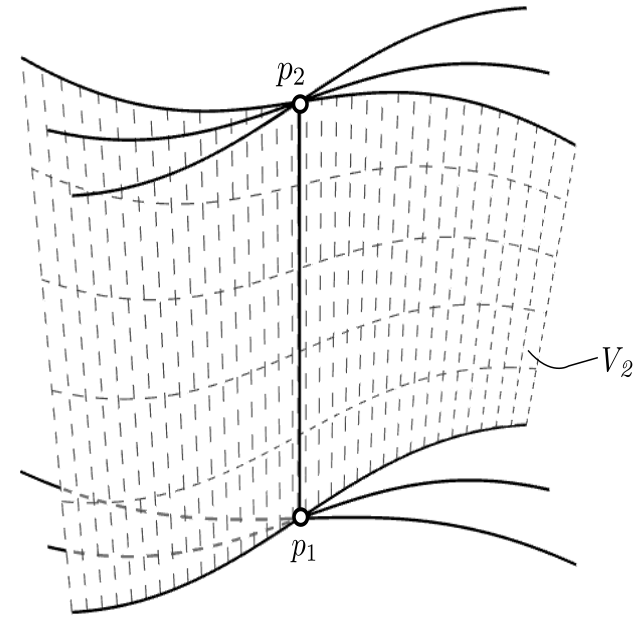
\includegraphics[width=6cm]{p87_a} }}%
    \qquad
    \subfloat[]{{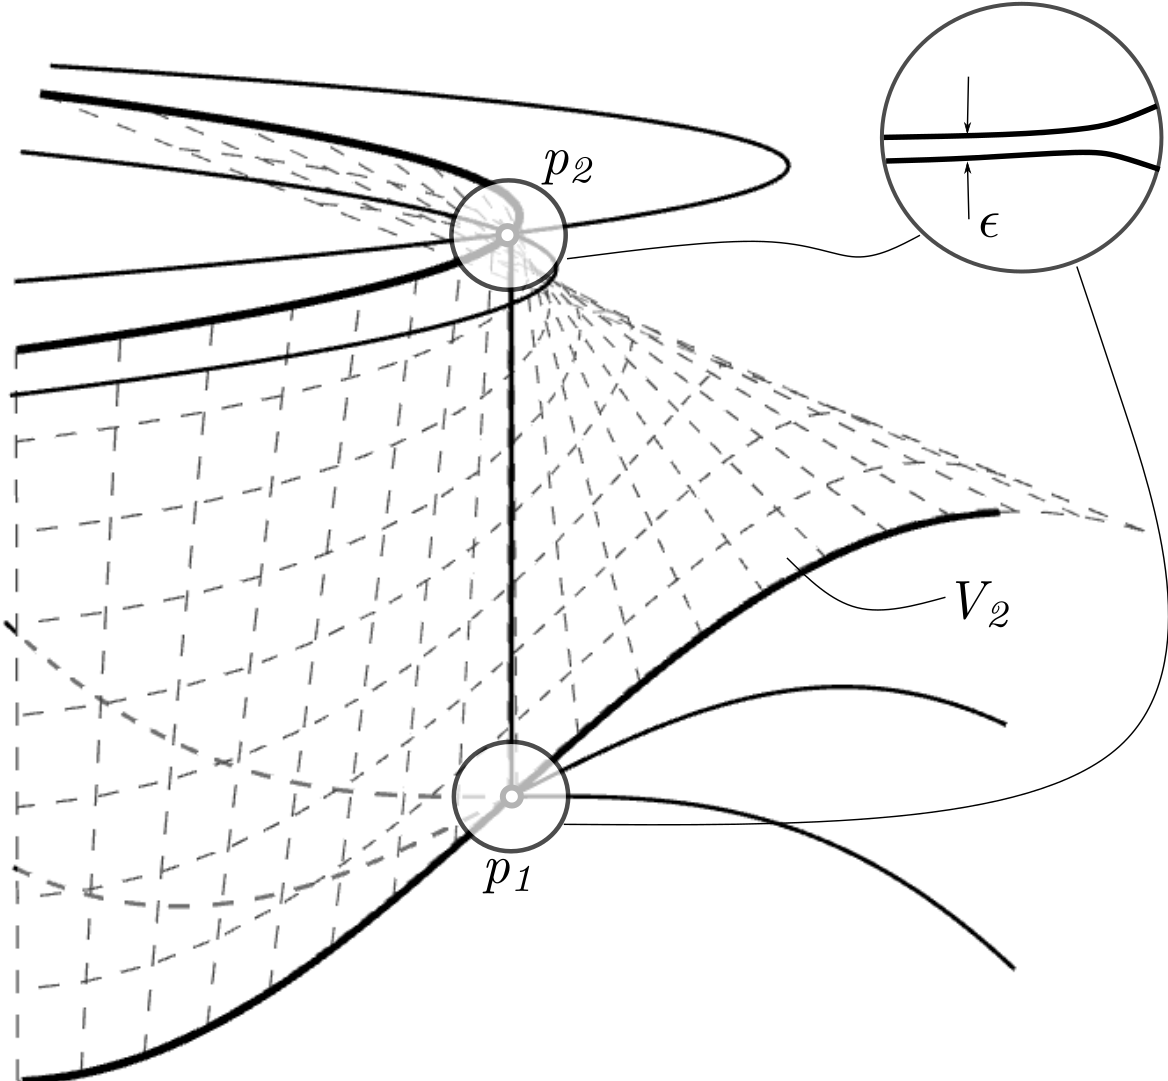
\includegraphics[width=6cm]{p87_c} }}%
        \qquad
    \subfloat[]{{\includegraphics[width=8cm]{p87_d} }}%
    %\caption{2 Figures side by side}%
    \label{fig:example}%
\caption{$V_2$ manifold of a family of geodesics}
\end{figure}
\begin{figure}[h]%
    \centering
\tdplotsetmaincoords{0}{10}
\pgfplotsset{every axis/.append style={
		scale=1,
		%axis lines=center,
		axis on top,
		xlabel={$x$},
		%ylabel={$z$},
               axis x line=middle,    % put the x axis in the middle
               axis y line=middle,    % put the y axis in the middle
               %x axis line style={-latex, ultra thin}, % arrows on the axis
               y axis line style={-,draw opacity=0},
                x axis line style={draw opacity=0},
            },}
            

            
\begin{tikzpicture}    [spy using outlines=	{circle, magnification=6, connect spies},] 
					
	\tikzmath{\u= 0.9;\w=-1.71;\v=1.0;\q= (2.0/ \w)*0.9994;\n=1;}
	\u,  \w, \v, \q, \n;
    \pgfplotsset{ticks=none};
    
    \pgfplotsset{compat=1.12};
		\def\r{0.5};
		\def\H{1.0};  
		\def\s{0.123};
	\begin{axis}
		[
		xmin=-0.7,
		xmax=0.7,
		ymin=-1.4,
		ymax=1.4,
		]
		%\addplot [black,thick,samples=1000,	samples y=0,	domain=-\r:\r,variable=\g]({ \r*(cos(\n*deg(2*ln(1-(\g)*\w/2))))},{(\u*(1-0.5*\g *\w)});
		%positve plane

		\addplot [decoration={markings,mark=at position 0.5 with {\arrow[scale=1,=>latex]{<}}},postaction={decorate}, black,thick,samples=60,	samples y=0,	domain=-\r:\r,variable=\g]({\g},{\u*(exp(0.5*(3.141593*(asin(\g/ \r)/360.-0.0))))});

		\addplot [black,dashed,thin,samples=40,	samples y=0,	domain=-\r:\r,variable=\g]({-\g},{\u*(exp(0.5*(3.141593*(asin(\g/ \r)/360.-0.5))))});
		%negative plane
		\addplot [decoration={markings,mark=at position 0.5 with {\arrow[scale=1.0,=>latex]{<}}},postaction={decorate},black,thick,samples=60,	samples y=0,	domain=-\r:\r,variable=\g]({\g},{-\u*(exp(0.5*(3.141593*(asin(\g/ \r)/360.-0.0))))});
		\addplot [black,dashed,thin,samples=40,	samples y=0,	domain=-\r:\r,variable=\g]({-\g},{-\u*(exp(0.5*(3.141593*(asin(\g/ \r)/360.-0.5))))});
		
		\foreach \k in {1,...,4}
{
%positve plane
  \addplot [black,very thick,samples=40,	samples y=0,	domain=-\r:\r,variable=\g]({\g},{\u*(exp(0.5*(3.141593*(asin(\g/ \r)/360.-\k ))))});
   \addplot [black,dashed,thin,samples=40,	samples y=0,	domain=-\r:\r,variable=\g]({-\g},{\u*(exp(0.5*(3.141593*(asin(\g/ \r)/360.-3*\k /2.))))});
  %negative plane
     \addplot [black,thick,samples=40,	samples y=0,	domain=-\r:\r,variable=\g]({\g},{-\u*(exp(0.5*(3.141593*(asin(\g/ \r)/360.-\k ))))});
   \addplot [black,dashed,thin,samples=40,	samples y=0,	domain=-\r:\r,variable=\g]({-\g},{-\u*(exp(0.5*(3.141593*(asin(\g/ \r)/360.-3*\k /2.))))});
}

      \coordinate (g1) at (axis cs:{\r*0.9},{\u*(exp(0.5*(3.141593*(asin(-\r/ \r)/360. +0.4))))});
      \coordinate (g2) at (axis cs:{\r*0.9},{-\u*(exp(0.5*(3.141593*(asin(-\r/ \r)/360.+0.4 ))))});
\node[tdplot_main_coords,{anchor=south east}] at (g1){$g_{1}$};
\node[tdplot_main_coords,{anchor=south east}] at (g2){$g_{2}$};

\foreach \j in {1,..,3}
{
%\draw (\j,0) -- (\j,\H*1.3);
}
\draw[very thin,] (\r,-\H*1.3) -- (\r,\H*1.3);
\draw[very thin,] (-\r,-\H*1.3) -- (-\r,\H*1.3);
\draw[thick,gray!60] (-\r,0) -- (\r,0);
\draw[very thin,black] (-\r,0) -- (\r,0);
\draw[very thin,black] (-\r*1.2,0) -- (-\r,0);
\draw[very thin,black,- stealth] (\r,0) -- (\r*1.42,0);


		%using the 'spy' to magnify a piece of the picture
  % now we can draw the magnifying glass:
    %\spy [black] on (2.84,2.87) in node [left] at (2.25,1.6);
      \coordinate (spypoint) at (axis cs:-0.493,0);
  \coordinate (magnifyglass) at (axis cs:-0.8,0.6);
\end{axis}
\spy [black, size=2.5cm] on (spypoint)   in node[fill=white] at (magnifyglass);

\end{tikzpicture}
\caption{$V_2$ Misner cylinder family of geodesics}
\end{figure}
$$\blacklozenge$$
\newpage

\end{comment}

\section{p96 - Clarification}
\begin{tcolorbox}
... But under parallel propagation along a geodesic, a vector makes a constant angle with the geodesic; following the vector round the small quadrilateral, it is easy to see that the angle through which the vector has turned on completion of the circuit is $E$, the excess of the angle-sum of four right angles...
\end{tcolorbox}
\begin{figure}[h]
            
\tikzmath{\dR=1.9;\da=-10.0;\dT=-0.59;\dD=-27.; \dV=-9.00;
\ra=7.5; \rb = \ra+\dR;
\rc=10.4; \rd = \rc+\dR;
\re=15.2; \rf = \re+0.1*\dR;
\rg=9.5; \rh = \rg+\dR;
\LNwee=0.5;
\LTree=1.3;
}

\begin{tikzpicture}[angle/.style={black,thick},]
\tdplotsetmaincoords{0}{10};
\pgfplotsset{every axis/.append style={
		view={-30*(0*1)}{-30*(-3)},
		%view={-90}{-30*0},
		scale=10/4,
		axis lines=center,
		%axis on top,
		%xlabel={$y$},
		%ylabel={$x$},
		%zlabel={$z$},
               %axis x line=middle,    % put the x axis in the middle
               %axis y line=middle,    % put the y axis in the middle
                %axis z line=middle,    % put the z axis in the middle
               %axis line style={-stealth}, % arrows on the axis
               axis line style={draw=none},
               axis equal image,
,
            }}
    \pgfplotsset{ticks=none};
    \pgfplotsset{compat=1.12};
	\begin{axis}[]
			
		%*******************************    first geodesics  ***********************************
		\addplot3 [thin,decoration={markings, mark = at position 0.39 with {\arrow[scale = 2.5]{latex[reversed]}}},postaction ={decorate},samples=40,	samples y=0,	domain=90.0+10:0-10]
		({-4.5+\ra*cos(x)},{-4.5+\ra*sin(x)},{0})node[above,left] {$\gamma_{1}$};
		
		
      		\def \f{19.6}%********************************************
      		
		\draw[fill=black]({-4.5+\ra*cos(\f)},{-4.5+\ra*sin(\f)},0) circle (3pt)node[{anchor=south west}] {$S$};;
     		\draw[very thick, -Latex]({-4.5+\ra*cos(\f)},{-4.5+\ra*sin(\f)},0) -- ({-4.5+\rb*cos(\f+\da)},{-4.5+\rb*sin(\f+\da)},0)node[below,right] {$\overrightarrow{u_{0}}$};
     		
      		\draw[-Latex,black] let
   		 \p0 = ({-4.5+\ra*cos(\f)},{-4.5+\ra*sin(\f)},0),
    		\p1 =  ({-4.5+\ra*cos(\f+\da)},{-4.5+\ra*sin(\f+\da)},0),
    		\p2 =  ({-4.5+\rb*cos(\f+\da)},{-4.5+\rb*sin(\f+\da)},0),
    		\n1 = {atan2(\y1 - \y0,\x1 - \x0)},
    		\n2 = {atan2(\y2 - \y0,\x2 - \x0)},
    		\n3 = {1.0cm},
    		\n4 = {(\n1 + \n2) / 2}
  		in ({-4.5+\ra*cos(\f)},{-4.5+\ra*sin(\f)},0) +(\n1:\n3) arc[radius = \n3, start angle = \n1, end angle = \n2]node[{anchor=north east}] {};;
  		
  		  \draw[black] let
   		\p0 = ({-4.5+\ra*cos(\f)},{-4.5+\ra*sin(\f)},0),
    		\p1 =  ( {-4.5+\ra*cos(\f-\da)},{-4.5+\ra*sin(\f-\da)},0) ,
    		\p2 =( {-4.5+\ra*cos(\f+\da)},{-4.5+\ra*sin(\f+\da)},0),
    		\n1 = {atan2(\y1 - \y0,\x1 - \x0)},
    		\n2 = {atan2(\y2 - \y0,\x2 - \x0)},
    		\n3 = {1.0cm},
    		\n4 = {(\n1 + \n2) / 2}
  		in ({-4.5+\ra*cos(\f)},{-4.5+\ra*sin(\f)},0) +(\n1:\n3) arc[radius = -\n3, start angle = \n2, end angle = \n1]node[midway,below,left] {$\theta_{1}$};;
  		
  		\def \ff{45}%********************************************
		\draw[very thick, -Latex]({-4.5+\ra*cos(\ff)},{-4.5+\ra*sin(\ff)},0) -- ({-4.5+\rb*cos(\ff+\da)},{-4.5+\rb*sin(\ff+\da)},0);

      		\draw[-Latex,black] let
   		 \p0 = ({-4.5+\ra*cos(\ff)},{-4.5+\ra*sin(\ff)},0),
    		\p1 =  ({-4.5+\ra*cos(\ff+\da)},{-4.5+\ra*sin(\ff+\da)},0),
    		\p2 =  ({-4.5+\rb*cos(\ff+\da)},{-4.5+\rb*sin(\ff+\da)},0),
    		\n1 = {atan2(\y1 - \y0,\x1 - \x0)},
    		\n2 = {atan2(\y2 - \y0,\x2 - \x0)},
    		\n3 = {0.6cm},
    		\n4 = {(\n1 + \n2) / 2}
  		in ({-4.5+\ra*cos(\ff)},{-4.5+\ra*sin(\ff)},0) +(\n1:\n3) arc[radius = \n3, start angle = \n1, end angle = \n2]node[midway,below] {};;
  		
  		 \draw[black] let
   		\p0 = ({-4.5+\ra*cos(\ff)},{-4.5+\ra*sin(\ff)},0),
    		\p1 =  ( {-4.5+\ra*cos(\ff-\da)},{-4.5+\ra*sin(\ff-\da)},0) ,
    		\p2 =( {-4.5+\ra*cos(\ff+\da)},{-4.5+\ra*sin(\ff+\da)},0),
    		\n1 = {atan2(\y1 - \y0,\x1 - \x0)},
    		\n2 = {atan2(\y2 - \y0,\x2 - \x0)},
    		\n3 = {0.6cm},
    		\n4 = {(\n1 + \n2) / 2}
  		in ({-4.5+\ra*cos(\ff)},{-4.5+\ra*sin(\ff)},0) +(\n1:\n3) arc[radius = -\n3, start angle = \n2, end angle = \n1]node[midway,below] {$\theta_{1} \ \ $};;
      		
      		\def \fff{77.2}%********************************************
		\draw[very thick, -Latex]({-4.5+\ra*cos(\fff)},{-4.5+\ra*sin(\fff)},0) -- ({-4.5+\rb*cos(\fff+\da)},{-4.5+\rb*sin(\fff+\da)},0);

		\draw[-Latex,black] let
   		\p0 = ({-4.5+\ra*cos(\fff)},{-4.5+\ra*sin(\fff)},0),
    		\p1 =   ( {-4.5+\ra*cos(\fff+\da)},{-4.5+\ra*sin(\fff+\da)},0),
    		\p2 = ({-4.5+\rb*cos(\fff+\da)},{-4.5+\rb*sin(\fff+\da)},0),
    		\n1 = {atan2(\y1 - \y0,\x1 - \x0)},
    		\n2 = {atan2(\y2 - \y0,\x2 - \x0)},
    		\n3 = {0.6cm},
    		\n4 = {(\n1 + \n2) / 2}
  		in ({-4.5+\ra*cos(\fff)},{-4.5+\ra*sin(\fff)},0) +(\n1:\n3) arc[radius = \n3, start angle = \n1, end angle = \n2]node[midway,below] {};;
  		
  		\draw[black] let
   		\p0 = ({-4.5+\ra*cos(\fff)},{-4.5+\ra*sin(\fff)},0),
    		\p1 =  ( {-4.5+\ra*cos(\fff-\da)},{-4.5+\ra*sin(\fff-\da)},0) ,
    		\p2 =( {-4.5+\ra*cos(\fff+\da)},{-4.5+\ra*sin(\fff+\da)},0),
    		\n1 = {atan2(\y1 - \y0,\x1 - \x0)},
    		\n2 = {atan2(\y2 - \y0,\x2 - \x0)},
    		\n3 = {0.6cm},
    		\n4 = {(\n1 + \n2) / 2}
  		in ({-4.5+\ra*cos(\fff)},{-4.5+\ra*sin(\fff)},0) +(\n1:\n3) arc[radius = -\n3, start angle = \n2, end angle = \n1]node[midway,below] {$\theta_{1} \ \ $};;
 		
 		 		
  		
  		%second geodesics **************************************
  			
		\addplot3 [thin,decoration={markings, mark = at position 0.4 with  {\arrow[scale = 2.5]{latex[reversed]}}},postaction ={decorate},samples=40,	samples y=0,	domain=300+80:295]({-9.1+\rg*cos(x)},{10+\rg*sin(x)},{0})node[below,left] {$\gamma_{2}$};
		
		\def\qt{2.55};

    		 \draw[-Latex,black] let
   		\p0 = ({-9.1+\rg*cos(\qt)},{10+\rg*sin(\qt)},0) ,
    		\p1 =   ({-9.1+\rg*cos(\qt+\dD)},{10+10.3*\rg*sin(\qt+\dD)},0) ,
    		\p2 =({-9.1+\rh*cos(\qt-\dD)},{10+\rh*sin(\qt-\dD)},0),
    		\n1 = {atan2(\y1 - \y0,\x1 - \x0)},
    		\n2 = {atan2(\y2 - \y0,\x2 - \x0)},
    		\n3 = {0.7cm},
    		\n4 = {(\n1 + \n2) / 3}
  		in ({-9.1+\rg*cos(\qt)},{10+\rg*sin(\qt)},0) +(\n1:\n3) arc[radius =- \n3, start angle = \n2, end angle = \n1]node[midway,{anchor=south east}] {$\theta_{2} \  $};;
      		
      		
      		\def\mt{-25};%***************************************************
 		
      		\draw[very thick, -Latex]({-9.1+\rg*cos(\mt)},{10+\rg*sin(\mt)},0) -- ({ (1-\LNwee)*(-9.1+\rg*cos(\mt))+\LNwee*(-9.1+(\rh*cos(\mt-\dD)))},{(1-\LNwee)*(10+\rg*sin(\mt))+\LNwee*(10+(\rh*sin(\mt-\dD)))},0)node[above,right] {};
      		
    		 \draw[-Latex,black] let
   		\p0 = ({-9.1+\rg*cos(\mt)},{10+\rg*sin(\mt)},0) ,
    		\p1 =   ({-9.1+\rg*cos(\mt+\dD)},{10+1.19*\rg*sin(\mt+\dD)},0) ,
    		\p2 =({-9.1+\rh*cos(\mt-\dD)},{10+\rh*sin(\mt-\dD)},0),
    		\n1 = {atan2(\y1 - \y0,\x1 - \x0)},
    		\n2 = {atan2(\y2 - \y0,\x2 - \x0)},
    		\n3 = {0.7cm},
    		\n4 = {(\n1 + \n2) / 3}
  		in ({-9.1+\rg*cos(\mt)},{10+\rg*sin(\mt)},0) +(\n1:\n3) arc[radius =- \n3, start angle = \n2, end angle = \n1]node[midway,above,left] {$\theta_{2} \ \ $};;     		
  		
  		
  		\def\mbt{-49};
  		
    		 \draw[-Latex,black] let
   		\p0 = ({-9.1+\rg*cos(\mbt)},{10+\rg*sin(\mbt)},0) ,
    		\p1 =   ({-9.1+\rg*cos(\mbt+\dD)},{10+1.1*\rg*sin(\mbt+\dD)},0) ,
    		\p2 =({-9.1+\rh*cos(\mbt-\dD)},{10+\rh*sin(\mbt-\dD)},0),
    		\n1 = {atan2(\y1 - \y0,\x1 - \x0)},
    		\n2 = {atan2(\y2 - \y0,\x2 - \x0)},
    		\n3 = {0.9cm},
    		\n4 = {(\n1 + \n2) / 3}
  		in ({-9.1+\rg*cos(\mbt)},{10+\rg*sin(\mbt)},0) +(\n1:\n3) arc[radius =- \n3, start angle = \n2, end angle = \n1]node[midway,above] {$\theta_{2} \ \ $};;

 		
 		
 		%***************************                           third geodesics                 *********************************
 		
		\addplot3 [thin,decoration={markings, mark = at position 0.5 with {\arrow[scale = 2.5]{latex[reversed]}}},postaction ={decorate},samples=40,	samples y=0,	domain=0-35:70.0+45]({\rc*cos(x)},{\rc*sin(x)},{0})node[below,left] {$\gamma_{3}$};
		
		\def\w{-15};
		\draw[very thick, -Latex]({\rc*cos(\w)},{\rc*sin(\w)},0) -- ({ (1-\LTree)*(\rc*cos(\w))+\LTree*((\rd*cos(\w+\dT)))},{(1-\LTree)*(\rc*sin(\w))+\LTree*(\rd*sin(\w+\dT))},0);
      		 \draw[-Latex,black] let
   		 \p0 = ({\rc*cos(\w)},{\rc*sin(\w)},0),
    		\p1 =  ({\rc*cos(\w+\dT)},{\rc*sin(\w+\dT)},0),
    		\p2 =  ({\rd*cos(\w+\dT)},{\rd*sin(\w+\dT)},0),
    		\n1 = {atan2(\y1 - \y0,\x1 - \x0)},
    		\n2 = {atan2(\y2 - \y0,\x2 - \x0)},
    		\n3 = {1.2cm},
    		\n4 = {(\n1 + \n2) / 2}
  		in ({\rc*cos(\w)},{\rc*sin(\w)},0) +(\n1:\n3) arc[radius = \n3, start angle = \n1, end angle = \n2]node[midway,below ] {$\ \ \theta_{3}$};
		
		\def \Tf{10}
		
		\draw[very thick, -Latex]({\rc*cos(\Tf)},{\rc*sin(\Tf)},0) -- ({ (1-\LTree)*(\rc*cos(\Tf))+\LTree*((\rd*cos(\Tf+\dT)))},{(1-\LTree)*(\rc*sin(\Tf))+\LTree*(\rd*sin(\Tf+\dT))},0);
      		\draw[-Latex,black] let
   		 \p0 = ({\rc*cos(\Tf)},{\rc*sin(\Tf)},0),
    		\p1 =  ({\rc*cos(\Tf+\dT)},{\rc*sin(\Tf+\dT)},0),
    		\p2 =  ({\rd*cos(\Tf+\dT)},{\rd*sin(\Tf+\dT)},0),
    		\n1 = {atan2(\y1 - \y0,\x1 - \x0)},
    		\n2 = {atan2(\y2 - \y0,\x2 - \x0)},
    		\n3 = {0.7cm},
    		\n4 = {(\n1 + \n2) / 2}
  		in ({\rc*cos(\Tf)},{\rc*sin(\Tf)},0) +(\n1:\n3) arc[radius = \n3, start angle = \n1, end angle = \n2]node[midway,below] {$\ \ \theta_{3}$};;
  
		\def \Ts{35}
      		\draw[very thick, -Latex]({\rc*cos(\Ts)},{\rc*sin(\Ts)},0) -- ({ (1-\LTree)*(\rc*cos(\Ts))+\LTree*((\rd*cos(\Ts+\dT)))},{(1-\LTree)*(\rc*sin(\Ts))+\LTree*(\rd*sin(\Ts+\dT))},0);
      		 \draw[-Latex,black] let
   		 \p0 = ({\rc*cos(\Ts)},{\rc*sin(\Ts)},0),
    		\p1 =  ({\rc*cos(\Ts+\dT)},{\rc*sin(\Ts+\dT)},0),
    		\p2 =  ({\rd*cos(\Ts+\dT)},{\rd*sin(\Ts+\dT)},0),
    		\n1 = {atan2(\y1 - \y0,\x1 - \x0)},
    		\n2 = {atan2(\y2 - \y0,\x2 - \x0)},
    		\n3 = {0.7cm},
    		\n4 = {(\n1 + \n2) / 2}
  		in ({\rc*cos(\Ts)},{\rc*sin(\Ts)},0) +(\n1:\n3) arc[radius = \n3, start angle = \n1, end angle = \n2]node[midway,right] {$\ \ \theta_{3}$};
      		
		\def \Tt{70}
      		\draw[very thick, -Latex]({\rc*cos(\Tt)},{\rc*sin(\Tt)},0) -- ({ (1-\LTree)*(\rc*cos(\Tt))+\LTree*((\rd*cos(\Tt+\dT)))},{(1-\LTree)*(\rc*sin(\Tt))+\LTree*(\rd*sin(\Tt+\dT))},0);
      		 \draw[-Latex,black] let
   		 \p0 = ({\rc*cos(\Tt)},{\rc*sin(\Tt)},0),
    		\p1 =  ({\rc*cos(\Tt+\dT)},{\rc*sin(\Tt+\dT)},0),
    		\p2 =  ({\rd*cos(\Tt+\dT)},{\rd*sin(\Tt+\dT)},0),
    		\n1 = {atan2(\y1 - \y0,\x1 - \x0)},
    		\n2 = {atan2(\y2 - \y0,\x2 - \x0)},
    		\n3 = {0.7cm},
    		\n4 = {(\n1 + \n2) / 2}
  		in ({\rc*cos(\Tt)},{\rc*sin(\Tt)},0) +(\n1:\n3) arc[radius = \n3, start angle = \n1, end angle = \n2]node[midway,right] {$  \ \ \theta_{3}$};
  		
  		
  		
  		\def\ww{88};
		\draw[very thick, -Latex]({\rc*cos(\ww)},{\rc*sin(\ww)},0) -- ({ (1-\LTree)*(\rc*cos(\ww))+\LTree*((\rd*cos(\ww+\dT)))},{(1-\LTree)*(\rc*sin(\ww))+\LTree*(\rd*sin(\ww+\dT))},0);
      		 \draw[-Latex,black] let
   		 \p0 = ({\rc*cos(\ww)},{\rc*sin(\ww)},0),
    		\p1 =  ({\rc*cos(\ww+\dT)},{\rc*sin(\ww+\dT)},0),
    		\p2 =  ({\rd*cos(\ww+\dT)},{\rd*sin(\ww+\dT)},0),
    		\n1 = {atan2(\y1 - \y0,\x1 - \x0)},
    		\n2 = {atan2(\y2 - \y0,\x2 - \x0)},
    		\n3 = {0.7cm},
    		\n4 = {(\n1 + \n2) / 2}
  		in ({\rc*cos(\ww)},{\rc*sin(\ww)},0) +(\n1:\n3) arc[radius = \n3, start angle = \n1, end angle = \n2]node[midway,right ] {$\ \ \theta_{3}$};
   
  				
  		%************************************************ fourth geodesics **************************************
  				
		\addplot3 [thin,decoration={markings, mark = at position 0.45 with {\arrow[scale = 2.5]{latex[reversed]}}},postaction ={decorate},samples=40,	samples y=0,	domain=270.0+20:270.0-30]({5-\re*cos(x)},{-17-\re*sin(x)},{0})node[below,left]  {$ \gamma_{4} \ $};
		
		\def\q{109.5};

    		 \draw[-Latex,black] let
   		\p0 = ({5-\re*cos(\q)},{-17+\re*sin(\q)},0) ,
    		\p1 =   ({5-\re*cos(\q+\dV)},{-17+\re*sin(\q+\dV)},0) ,
    		\p2 =({5-\rf*cos(\q-\dV)},{-17+\rf*sin(\q-\dV)},0),
    		\n1 = {atan2(\y1 - \y0,\x1 - \x0)},
    		\n2 = {atan2(\y2 - \y0,\x2 - \x0)},
    		\n3 = {0.6cm},
    		\n4 = {(\n1 + \n2) / 3}
  		in ({5-\re*cos(\q)},{-17+\re*sin(\q)},0) +(\n1:\n3) arc[radius =- \n3, start angle = \n2, end angle = \n1]node[midway,left,below] {$\ \ \ \theta_{4} $};;
      		
      		
      		\def\m{95};%***************************************************
		
      		\draw[very thick, -Latex]({5-\re*cos(\m)},{-17+\re*sin(\m)},0) -- ({1*(5-\rf*cos(\m-\dV))},{1*(-17+\rf*sin(\m-\dV))},0)node[right] {};;

    		 \draw[-Latex,black] let
   		\p0 = ({5-\re*cos(\m)},{-17+\re*sin(\m)},0) ,
    		\p1 =   ({5-\re*cos(\m+\dV)},{-17+\re*sin(\m+\dV)},0) ,
    		\p2 =({5-\rf*cos(\m-\dV)},{-17+\rf*sin(\m-\dV)},0),
    		\n1 = {atan2(\y1 - \y0,\x1 - \x0)},
    		\n2 = {atan2(\y2 - \y0,\x2 - \x0)},
    		\n3 = {0.4cm},
    		\n4 = {(\n1 + \n2) / 3}
  		in ({5-\re*cos(\m)},{-17+\re*sin(\m)},0) +(\n1:\n3) arc[radius =- \n3, start angle = \n2, end angle = \n1]node[midway,below] {$\theta_{4} \ \ \ $};;
      		
  		\def\mb{81};
		
      		\draw[very thick, -Latex]({5-\re*cos(\mb)},{-17+\re*sin(\mb)},0) -- ({5-\rf*cos(\mb-\dV)},{-17+\rf*sin(\mb-\dV)},0)node[{anchor=south west}] {$\overrightarrow{u_{t}}$};;

    		 \draw[-Latex,black] let
   		\p0 = ({5-\re*cos(\mb)},{-17+\re*sin(\mb)},0) ,
    		\p1 =   ({5-\re*cos(\mb+\dV)},{-17+\re*sin(\mb+\dV)},0) ,
    		\p2 =({5-\rf*cos(\mb-\dV)},{-17+\rf*sin(\mb-\dV)},0),
    		\n1 = {atan2(\y1 - \y0,\x1 - \x0)},
    		\n2 = {atan2(\y2 - \y0,\x2 - \x0)},
    		\n3 = {0.8cm},
    		\n4 = {(\n1 + \n2) / 3}
  		in ({5-\re*cos(\mb)},{-17+\re*sin(\mb)},0) +(\n1:\n3) arc[radius = \n3, start angle = \n1, end angle = \n2]node[midway,below,left] {$\theta_{4} \ \ \ \ $};;
  		
  %********************* angle between begin and end vector

    		      	\draw[Latex-Latex,black,  thick] let
   		 \p0 = ({-4.5+\ra*cos(\f)},{-4.5+\ra*sin(\f)},0),
    		\p1 =   ({5+\re*cos(\mb+\dV)},{-17+1.1*\re*sin(\mb+\dV)},0) ,
    		\p2 =  ({-4.5+\rb*cos(\f+\da)},{-4.5+\rb*sin(\f+\da)},0),
    		\n1 = {atan2(\y1 - \y0,\x1 - \x0)},
    		\n2 = {atan2(\y2 - \y0,\x2 - \x0)},
    		\n3 = {1.4cm},
    		\n4 = {(\n1 + \n2) / 2}
  		in ({-4.5+\ra*cos(\f)},{-4.5+\ra*sin(\f)},0) +(\n1:\n3) arc[radius = \n3, start angle = \n1, end angle = \n2]node[midway,below,right] {$\delta\theta$};;

%********************* angles between the 4 geodesic paths
				% ***************************** 1 and 4 *************************
					
	  	\draw[-Latex,dashed,black,  thick] let
   		 \p0 = ({-4.5+\ra*cos(\f)},{-4.5+\ra*sin(\f)},0),
    		\p1 =   ({5+\re*cos(\mb+\dV)},{-17+1.1*\re*sin(\mb+\dV)},0) ,
    		\p2 =  ({-4.5+\ra*cos(\f-\da)},{-4.5+\ra*sin(\f-\da)},0),
    		\n1 = {atan2(\y1 - \y0,\x1 - \x0)},
    		\n2 = {atan2(\y2 - \y0,\x2 - \x0)},
    		\n3 = {1.0cm},
    		\n4 = {(\n1 + \n2) / 2}
  		in ({-4.5+\ra*cos(\f)},{-4.5+\ra*sin(\f)},0) +(\n1:\n3) arc[radius = \n3, start angle = \n1, end angle = \n2]node[midway,below,right] {$\ \ \Psi_{4\rightarrow 1}$};;
				
				% ***************************** 1 and 2 *************************
					
	  	\draw[-Latex,dashed,black,  thick] let
   		\p0 = ({-4.5+\ra*cos(\fff)},{-4.5+\ra*sin(\fff)},0),
    		\p1 =   ( {-4.5+\ra*cos(\fff+\da)},{-4.5+\ra*sin(\fff+\da)},0),
    		\p2 =({-9.1+\rg*cos(\mbt-\dD)},{10+1.19*\rg*sin(\mbt-\dD)},0),
    		\n1 = {atan2(\y1 - \y0,\x1 - \x0)},
    		\n2 = {atan2(\y2 - \y0,\x2 - \x0)},
    		\n3 = {1.2cm},
    		\n4 = {(\n1 + \n2) / 2}
  		in ({-4.5+\ra*cos(\fff)},{-4.5+\ra*sin(\fff)},0) +(\n1:\n3) arc[radius = \n3, start angle = \n1, end angle = \n2]node[midway,right]{$\  \ \Psi_{1\rightarrow 2}$};		
				
				% ***************************** 2 and 3  *************************
		 \draw[-Latex,dashed,black,  thick] let
   		 \p0 = ({\rc*cos(\ww)},{\rc*sin(\ww)},0),
    		\p1 =   ({-9.1+1.1*\rg*cos(\qt+\dD)},{10+1.1*\rg*sin(\qt+\dD)},0) ,
    		\p2 =  ({\rc*cos(\ww+\dT)},{\rc*sin(\ww+\dT)},0),
    		\n1 = {atan2(\y1 - \y0,\x1 - \x0)},
    		\n2 = {atan2(\y2 - \y0,\x2 - \x0)},
    		\n3 = {0.8cm},
    		\n4 = {(\n1 + \n2) / 2}
  		in ({\rc*cos(\ww)},{\rc*sin(\ww)},0) +(\n1:\n3) arc[radius = \n3, start angle = \n1, end angle = \n2]node[midway,right ] {$\  \ \Psi_{2\rightarrow 3}$};	
			
			
						% ***************************** 3 and 4  *************************
		 \draw[-Latex,dashed,black,  thick] let
   		 \p0 = ({\rc*cos(\w)},{\rc*sin(\w)},0),
    		\p1 =  ({\rc*cos(\w+\dT)},{1.04*\rc*sin(\w+\dT)},0),
    		\p2 =({5-\rf*cos(\q-\dV)},{-17+\rf*sin(\q-\dV)},0),
    		\n1 = {atan2(\y1 - \y0,\x1 - \x0)},
    		\n2 = {atan2(\y2 - \y0,\x2 - \x0)},
    		\n3 = {-0.8cm},
    		\n4 = {(\n1 + \n2) / 2}
  		in ({\rc*cos(\w)},{\rc*sin(\w)},0) +(\n1:\n3) arc[radius = \n3, start angle = \n1, end angle = \n2]node[midway,above, ] {$ \Psi_{3\rightarrow 4} \ \ \ \ \ $};	
			
\end{axis}
\end{tikzpicture}\\
\caption{Parallel transportation along a  closed path}
\end{figure}
Consider 4 geodesics $\gamma_{1}, \gamma_{2},\gamma_{3},\gamma_{4}$ close to each other so that they form a small quadrilateral. At each intersection they form an angle $\Psi_{i\rightarrow i+1}$. A vector $\overrightarrow{u_{0}}$ is transported parallely along the path starting at the intersection $S$ of $\gamma_{1},\gamma_{4}$ and ends as vector $\overrightarrow{u_{t}}$ at the same point $S$. In general $\overrightarrow{u_{0}}\ne \overrightarrow{u_{t}}$ and will differ by a small angle $\delta\theta$. Let's investigate the relationship between $\delta\theta$ and the $\Psi_{i\rightarrow i+1}$.\\
\begin{figure}[h]
  
\tikzmath{\dR=1.9;\da=-10.0;\dT=-0.59;\dD=-27.; \dV=-9.00;
\ra=7.5; \rb = \ra+\dR;
\rc=10.4; \rd = \rc+\dR;
\re=15.2; \rf = \re+0.1*\dR;
\rg=9.5; \rh = \rg+\dR;
\LNwee=0.5;
\LTree=1.3;
}

            
\begin{tikzpicture}[angle/.style={black,thick},]
\tdplotsetmaincoords{0}{10};
\pgfplotsset{every axis/.append style={
		view={-30*(0*1)}{-30*(-3)},
		%view={-90}{-30*0},
		scale=10/4,
		axis lines=center,
		%axis on top,
		%xlabel={$y$},
		%ylabel={$x$},
		%zlabel={$z$},
               %axis x line=middle,    % put the x axis in the middle
               %axis y line=middle,    % put the y axis in the middle
                %axis z line=middle,    % put the z axis in the middle
               %axis line style={-stealth}, % arrows on the axis
               axis line style={draw=none},
               axis equal image,
,
            }}
    \pgfplotsset{ticks=none};
    \pgfplotsset{compat=1.12};
	\begin{axis}[]
			
		%*******************************    first geodesics  ***********************************
		\addplot3 [dashed,thin,decoration={markings, mark = at position 0.5 with {\arrow[scale = 2.5]{latex[reversed]}}},postaction ={decorate},samples=40,	samples y=0,	domain=90.0+10:0-10]
		({-4.5+\ra*cos(x)},{-4.5+\ra*sin(x)},{0})node[above,left] {$T(\gamma_{1})$};
		
		
      		\def \f{19.6}%********************************************
      		\def\fe{-2}
		\draw[fill=black]({-4.5+\ra*cos(\f)},{-4.5+\ra*sin(\f)},0) circle (3pt)node[{anchor=south west}] {$S$};;
     		\draw[very thin, -Latex]({-4.5+\ra*cos(\f)},{-4.5+\ra*sin(\f)},0) -- ({-4.5+\rb*cos(\f+\da)},{-4.5+\rb*sin(\f+\da)},0)node[below,right] {$\overrightarrow{u_{0}}$};
     		\draw[very thick, -Latex]({-4.5+\ra*cos(\f)},{-4.5+\ra*sin(\f)},0) -- ({(1-\fe)*(-4.5+\ra*cos(\f))+1.09*\fe*(-4.5+\ra*cos(\f+\da))},{(1-\fe)*(-4.5+\ra*sin(\f))+\fe*(-4.5+\ra*sin(\f+\da))},0)node[{anchor=south west}] {$\overrightarrow{\xi_{1}}$};
      		\draw[-Latex,black,thin] let
   		 \p0 = ({-4.5+\ra*cos(\f)},{-4.5+\ra*sin(\f)},0),
    		\p1 =  ({-4.5+\ra*cos(\f+\da)},{-4.5+\ra*sin(\f+\da)},0),
    		\p2 =  ({-4.5+\rb*cos(\f+\da)},{-4.5+\rb*sin(\f+\da)},0),
    		\n1 = {atan2(\y1 - \y0,\x1 - \x0)},
    		\n2 = {atan2(\y2 - \y0,\x2 - \x0)},
    		\n3 = {1.0cm},
    		\n4 = {(\n1 + \n2) / 2}
  		in ({-4.5+\ra*cos(\f)},{-4.5+\ra*sin(\f)},0) +(\n1:\n3) arc[radius = \n3, start angle = \n1, end angle = \n2]node[{anchor=north east}] {};;
  		
  		  \draw[black,thin] let
   		\p0 = ({-4.5+\ra*cos(\f)},{-4.5+\ra*sin(\f)},0),
    		\p1 =  ( {-4.5+\ra*cos(\f-\da)},{-4.5+\ra*sin(\f-\da)},0) ,
    		\p2 =( {-4.5+\ra*cos(\f+\da)},{-4.5+\ra*sin(\f+\da)},0),
    		\n1 = {atan2(\y1 - \y0,\x1 - \x0)},
    		\n2 = {atan2(\y2 - \y0,\x2 - \x0)},
    		\n3 = {1.0cm},
    		\n4 = {(\n1 + \n2) / 2}
  		in ({-4.5+\ra*cos(\f)},{-4.5+\ra*sin(\f)},0) +(\n1:\n3) arc[radius = -\n3, start angle = \n2, end angle = \n1]node[{anchor=north east}] {$\theta_{1}$};;
  		
  	
      		\def \fff{77.2}%********************************************
		\draw[thin, -Latex]({-4.5+\ra*cos(\fff)},{-4.5+\ra*sin(\fff)},0) -- ({-4.5+\rb*cos(\fff+\da)},{-4.5+\rb*sin(\fff+\da)},0);

		\draw[-Latex,black,thin] let
   		\p0 = ({-4.5+\ra*cos(\fff)},{-4.5+\ra*sin(\fff)},0),
    		\p1 =   ( {-4.5+\ra*cos(\fff+\da)},{-4.5+\ra*sin(\fff+\da)},0),
    		\p2 = ({-4.5+\rb*cos(\fff+\da)},{-4.5+\rb*sin(\fff+\da)},0),
    		\n1 = {atan2(\y1 - \y0,\x1 - \x0)},
    		\n2 = {atan2(\y2 - \y0,\x2 - \x0)},
    		\n3 = {0.6cm},
    		\n4 = {(\n1 + \n2) / 2}
  		in ({-4.5+\ra*cos(\fff)},{-4.5+\ra*sin(\fff)},0) +(\n1:\n3) arc[radius = \n3, start angle = \n1, end angle = \n2]node[midway,below] {};;
  		
  		\draw[black,thin] let
   		\p0 = ({-4.5+\ra*cos(\fff)},{-4.5+\ra*sin(\fff)},0),
    		\p1 =  ( {-4.5+\ra*cos(\fff-\da)},{-4.5+\ra*sin(\fff-\da)},0) ,
    		\p2 =( {-4.5+\ra*cos(\fff+\da)},{-4.5+\ra*sin(\fff+\da)},0),
    		\n1 = {atan2(\y1 - \y0,\x1 - \x0)},
    		\n2 = {atan2(\y2 - \y0,\x2 - \x0)},
    		\n3 = {0.6cm},
    		\n4 = {(\n1 + \n2) / 2}
  		in ({-4.5+\ra*cos(\fff)},{-4.5+\ra*sin(\fff)},0) +(\n1:\n3) arc[radius = -\n3, start angle = \n2, end angle = \n1]node[midway,below] {$\theta_{1} \ \ $};;
 		
 		 \draw[very thick, -Latex]({-4.5+\ra*cos(\fff)},{-4.5+\ra*sin(\fff)},0) -- ({(1-\fe)*(-4.5+\ra*cos(\fff))+\fe*(-4.5+\ra*cos(\fff+\da))},{(1-\fe)*(-4.5+\ra*sin(\fff))+\fe*(-4.5+\ra*sin(\fff+\da))},0)node[{anchor=south west}]  {$\overrightarrow{\xi^{o}_{1}}$};		
  		
  		%second geodesics **************************************
  			
		\addplot3 [dashed,thin,decoration={markings, mark = at position 0.5 with  {\arrow[scale = 2.5]{latex[reversed]}}},postaction ={decorate},samples=40,	samples y=0,	domain=300+80:295]({-9.1+\rg*cos(x)},{10+\rg*sin(x)},{0})node[below,left] {$\gamma_{2}$};
		
		\def\qt{2.55};

    		 \draw[-Latex,black,thin] let
   		\p0 = ({-9.1+\rg*cos(\qt)},{10+\rg*sin(\qt)},0) ,
    		\p1 =   ({-9.1+\rg*cos(\qt+\dD)},{10+10.3*\rg*sin(\qt+\dD)},0) ,
    		\p2 =({-9.1+\rh*cos(\qt-\dD)},{10+\rh*sin(\qt-\dD)},0),
    		\n1 = {atan2(\y1 - \y0,\x1 - \x0)},
    		\n2 = {atan2(\y2 - \y0,\x2 - \x0)},
    		\n3 = {0.7cm},
    		\n4 = {(\n1 + \n2) / 3}
  		in ({-9.1+\rg*cos(\qt)},{10+\rg*sin(\qt)},0) +(\n1:\n3) arc[radius =- \n3, start angle = \n2, end angle = \n1]node[midway,{anchor=south east}] {$\theta_{2} \  $};;
      		\def \fed{-0.65};
 		\draw[very thick, -Latex]({-9.1+\rg*cos(\qt)},{10+\rg*sin(\qt)},0) -- ({(1-\fed)*(-9.1+\rg*cos(\qt))+\fed*(-9.1+1.15*\rg*cos(\qt+\dD))},{(1-\fed)*(10+\rg*sin(\qt))+\fed*(10+\rg*sin(\qt+\dD))},0)node[{anchor=north east}] {$\overrightarrow{\xi^{o}_{2}}$};
 		
      		
      		
  		\def\mbt{-49};
  		
    		 \draw[-Latex,black,thin] let
   		\p0 = ({-9.1+\rg*cos(\mbt)},{10+\rg*sin(\mbt)},0) ,
    		\p1 =   ({-9.1+\rg*cos(\mbt+\dD)},{10+1.1*\rg*sin(\mbt+\dD)},0) ,
    		\p2 =({-9.1+\rh*cos(\mbt-\dD)},{10+\rh*sin(\mbt-\dD)},0),
    		\n1 = {atan2(\y1 - \y0,\x1 - \x0)},
    		\n2 = {atan2(\y2 - \y0,\x2 - \x0)},
    		\n3 = {0.9cm},
    		\n4 = {(\n1 + \n2) / 3}
  		in ({-9.1+\rg*cos(\mbt)},{10+\rg*sin(\mbt)},0) +(\n1:\n3) arc[radius =- \n3, start angle = \n2, end angle = \n1]node[midway,above] {$\theta_{2} \ \ $};;
		\def \fet{-0.47};
 		\draw[very thick, -Latex]({-9.1+\rg*cos(\mbt)},{10+\rg*sin(\mbt)},0) -- ({(1-\fet)*(-9.1+\rg*cos(\mbt))+\fet*(-9.1+\rg*cos(\mbt+\dD))},{(1-\fet)*(10+\rg*sin(\mbt))+\fet*(10+1.2*\rg*sin(\mbt+\dD))},0)node[below,right] {$\overrightarrow{\xi_{2}}$};
 		
 		%***************************                           third geodesics                 *********************************
 		
		\addplot3 [dashed,thin,decoration={markings, mark = at position 0.5 with {\arrow[scale = 2.5]{latex[reversed]}}},postaction ={decorate},samples=40,	samples y=0,	domain=0-35:70.0+45]({\rc*cos(x)},{\rc*sin(x)},{0})node[below,left] {$\gamma_{3}$};
		
		\def\w{-15};
		\draw[thin, -Latex]({\rc*cos(\w)},{\rc*sin(\w)},0) -- ({ (1-\LTree)*(\rc*cos(\w))+\LTree*((\rd*cos(\w+\dT)))},{(1-\LTree)*(\rc*sin(\w))+\LTree*(\rd*sin(\w+\dT))},0);
      		 \draw[-Latex,black,thin] let
   		 \p0 = ({\rc*cos(\w)},{\rc*sin(\w)},0),
    		\p1 =  ({\rc*cos(\w+\dT)},{\rc*sin(\w+\dT)},0),
    		\p2 =  ({\rd*cos(\w+\dT)},{\rd*sin(\w+\dT)},0),
    		\n1 = {atan2(\y1 - \y0,\x1 - \x0)},
    		\n2 = {atan2(\y2 - \y0,\x2 - \x0)},
    		\n3 = {1.2cm},
    		\n4 = {(\n1 + \n2) / 2}
  		in ({\rc*cos(\w)},{\rc*sin(\w)},0) +(\n1:\n3) arc[radius = \n3, start angle = \n1, end angle = \n2]node[midway,below ] {$\ \ \theta_{3}$};
		
		\def \tho{0.47};
 		\draw[very thick, -Latex]({-9.1*0+\rc*cos(\w)},{10*0+\rc*sin(\w)},0) -- ({(1-\tho)*(-9.1*0+\rc*cos(\w))+1.1*\tho*(-9.1*0+\rc*cos(\w+\dD))},{(1-\tho)*(10*0+\rc*sin(\w))+\tho*(10*0+1.2*\rc*sin(\w+\dD))},0)node[below,right] {$\overrightarrow{\xi^{o}_{3}}$};
  		
  		\def\ww{88};
		\draw[thin, -Latex]({\rc*cos(\ww)},{\rc*sin(\ww)},0) -- ({ (1-\LTree)*(\rc*cos(\ww))+\LTree*((\rd*cos(\ww+\dT)))},{(1-\LTree)*(\rc*sin(\ww))+\LTree*(\rd*sin(\ww+\dT))},0);
      		 \draw[-Latex,black,thin] let
   		 \p0 = ({\rc*cos(\ww)},{\rc*sin(\ww)},0),
    		\p1 =  ({\rc*cos(\ww+\dT)},{\rc*sin(\ww+\dT)},0),
    		\p2 =  ({\rd*cos(\ww+\dT)},{\rd*sin(\ww+\dT)},0),
    		\n1 = {atan2(\y1 - \y0,\x1 - \x0)},
    		\n2 = {atan2(\y2 - \y0,\x2 - \x0)},
    		\n3 = {0.7cm},
    		\n4 = {(\n1 + \n2) / 2}
  		in ({\rc*cos(\ww)},{\rc*sin(\ww)},0) +(\n1:\n3) arc[radius = \n3, start angle = \n1, end angle = \n2]node[midway,right ] {$\ \ \theta_{3}$};
   		\def \tht{0.57};
 		\draw[very thick, -Latex]({-9.1*0+\rc*cos(\ww)},{10*0+\rc*sin(\ww)},0) -- ({(1-\tht)*(-9.1*0+\rc*cos(\ww))+\tht*(-9.1*0+\rc*cos(\ww+\dD))},{(1-\tht)*(10*0+\rc*sin(\ww))+\tht*(10*0+1.1*\rc*sin(\ww+\dD))},0)node[below,right] {$\overrightarrow{\xi_{3}}$};
  				
  		%************************************************ fourth geodesics **************************************
  				
		\addplot3 [dashed,thin,decoration={markings, mark = at position 0.5 with {\arrow[scale = 2.5]{latex[reversed]}}},postaction ={decorate},samples=40,	samples y=0,	domain=270.0+20:270.0-30]({5-\re*cos(x)},{-17-\re*sin(x)},{0})node[below,left] {$ \gamma_{4} \ $};
		
		\def\q{109.5};

    		 \draw[-Latex,black,thin] let
   		\p0 = ({5-\re*cos(\q)},{-17+\re*sin(\q)},0) ,
    		\p1 =   ({5-\re*cos(\q+\dV)},{-17+\re*sin(\q+\dV)},0) ,
    		\p2 =({5-\rf*cos(\q-\dV)},{-17+\rf*sin(\q-\dV)},0),
    		\n1 = {atan2(\y1 - \y0,\x1 - \x0)},
    		\n2 = {atan2(\y2 - \y0,\x2 - \x0)},
    		\n3 = {0.6cm},
    		\n4 = {(\n1 + \n2) / 3}
  		in ({5-\re*cos(\q)},{-17+\re*sin(\q)},0) +(\n1:\n3) arc[radius =- \n3, start angle = \n2, end angle = \n1]node[midway,left,below] {$\ \ \ \theta_{4} $};;
      		\def\fto{1};
      		\draw[very thick, -Latex]({5-\re*cos(\q)},{-17+\re*sin(\q)},0) -- ({(1-\fto)*(5-\re*cos(\q))+\fto*(5-\re*cos(\q+\dV))},{(1-\fto)*(-17+\re*sin(\q))+\fto*(-17+\re*sin(\q+\dV))},0)node[{anchor=south east}] {$\overrightarrow{\xi_{4}}$};
      		
  		\def\mb{81};
		
      		\draw[thin, -Latex]({5-\re*cos(\mb)},{-17+\re*sin(\mb)},0) -- ({5-\rf*cos(\mb-\dV)},{-17+\rf*sin(\mb-\dV)},0)node[{anchor=south west}] {$\overrightarrow{u_{t}}$};;

    		 \draw[-Latex,black,thin] let
   		\p0 = ({5-\re*cos(\mb)},{-17+\re*sin(\mb)},0) ,
    		\p1 =   ({5-\re*cos(\mb+\dV)},{-17+\re*sin(\mb+\dV)},0) ,
    		\p2 =({5-\rf*cos(\mb-\dV)},{-17+\rf*sin(\mb-\dV)},0),
    		\n1 = {atan2(\y1 - \y0,\x1 - \x0)},
    		\n2 = {atan2(\y2 - \y0,\x2 - \x0)},
    		\n3 = {0.8cm},
    		\n4 = {(\n1 + \n2) / 3}
  		in ({5-\re*cos(\mb)},{-17+\re*sin(\mb)},0) +(\n1:\n3) arc[radius = \n3, start angle = \n1, end angle = \n2]node[midway,below,left] {$\theta_{4} \ \ \ \ $};;
  		\def\fttw{1.2};
      	\draw[very thick, -Latex]({5-\re*cos(\mb)},{-17+\re*sin(\mb)},0) -- ({(1-\fttw)*(5-\re*cos(\mb))+\fttw*(5-\re*cos(\mb+\dV))},{(1-\fttw)*(-17+\re*sin(\mb))+\fttw*(-17+\re*sin(\mb+\dV))},0)node[{anchor=south west}] {$\overrightarrow{\xi^{o}_{4}}$};
  %********************* angle between begin and end vector

    		      	\draw[Latex-Latex,black,  thin] let
   		 \p0 = ({-4.5+\ra*cos(\f)},{-4.5+\ra*sin(\f)},0),
    		\p1 =   ({5+\re*cos(\mb+\dV)},{-17+1.1*\re*sin(\mb+\dV)},0) ,
    		\p2 =  ({-4.5+\rb*cos(\f+\da)},{-4.5+\rb*sin(\f+\da)},0),
    		\n1 = {atan2(\y1 - \y0,\x1 - \x0)},
    		\n2 = {atan2(\y2 - \y0,\x2 - \x0)},
    		\n3 = {1.4cm},
    		\n4 = {(\n1 + \n2) / 2}
  		in ({-4.5+\ra*cos(\f)},{-4.5+\ra*sin(\f)},0) +(\n1:\n3) arc[radius = \n3, start angle = \n1, end angle = \n2]node[midway,below,right] {$\delta\theta$};;

%********************* angles between the 4 geodesic paths
				% ***************************** 1 and 4 *************************
					
	  	\draw[-Latex,dashed,black,  thin] let
   		 \p0 = ({-4.5+\ra*cos(\f)},{-4.5+\ra*sin(\f)},0),
    		\p1 =   ({5+\re*cos(\mb+\dV)},{-17+1.1*\re*sin(\mb+\dV)},0) ,
    		\p2 =  ({-4.5+\ra*cos(\f-\da)},{-4.5+\ra*sin(\f-\da)},0),
    		\n1 = {atan2(\y1 - \y0,\x1 - \x0)},
    		\n2 = {atan2(\y2 - \y0,\x2 - \x0)},
    		\n3 = {1.0cm},
    		\n4 = {(\n1 + \n2) / 2}
  		in ({-4.5+\ra*cos(\f)},{-4.5+\ra*sin(\f)},0) +(\n1:\n3) arc[radius = \n3, start angle = \n1, end angle = \n2]node[midway,below,right] {$\ \ \Psi_{4\rightarrow 1}$};;
				
				% ***************************** 1 and 2 *************************
					
	  	\draw[-Latex,dashed,black,  thin] let
   		\p0 = ({-4.5+\ra*cos(\fff)},{-4.5+\ra*sin(\fff)},0),
    		\p1 =   ( {-4.5+\ra*cos(\fff+\da)},{-4.5+\ra*sin(\fff+\da)},0),
    		\p2 =({-9.1+\rg*cos(\mbt-\dD)},{10+1.19*\rg*sin(\mbt-\dD)},0),
    		\n1 = {atan2(\y1 - \y0,\x1 - \x0)},
    		\n2 = {atan2(\y2 - \y0,\x2 - \x0)},
    		\n3 = {1.2cm},
    		\n4 = {(\n1 + \n2) / 2}
  		in ({-4.5+\ra*cos(\fff)},{-4.5+\ra*sin(\fff)},0) +(\n1:\n3) arc[radius = \n3, start angle = \n1, end angle = \n2]node[midway,right]{$\  \ \Psi_{1\rightarrow 2}$};		
				
				% ***************************** 2 and 3  *************************
		 \draw[-Latex,dashed,black,  thin] let
   		 \p0 = ({\rc*cos(\ww)},{\rc*sin(\ww)},0),
    		\p1 =   ({-9.1+1.1*\rg*cos(\qt+\dD)},{10+1.1*\rg*sin(\qt+\dD)},0) ,
    		\p2 =  ({\rc*cos(\ww+\dT)},{\rc*sin(\ww+\dT)},0),
    		\n1 = {atan2(\y1 - \y0,\x1 - \x0)},
    		\n2 = {atan2(\y2 - \y0,\x2 - \x0)},
    		\n3 = {0.8cm},
    		\n4 = {(\n1 + \n2) / 2}
  		in ({\rc*cos(\ww)},{\rc*sin(\ww)},0) +(\n1:\n3) arc[radius = \n3, start angle = \n1, end angle = \n2]node[midway,right ] {$\  \ \Psi_{2\rightarrow 3}$};	
			
			
						% ***************************** 3 and 4  *************************
		 \draw[-Latex,dashed,black,  thin] let
   		 \p0 = ({\rc*cos(\w)},{\rc*sin(\w)},0),
    		\p1 =  ({\rc*cos(\w+\dT)},{1.04*\rc*sin(\w+\dT)},0),
    		\p2 =({5-\rf*cos(\q-\dV)},{-17+\rf*sin(\q-\dV)},0),
    		\n1 = {atan2(\y1 - \y0,\x1 - \x0)},
    		\n2 = {atan2(\y2 - \y0,\x2 - \x0)},
    		\n3 = {-0.8cm},
    		\n4 = {(\n1 + \n2) / 2}
  		in ({\rc*cos(\w)},{\rc*sin(\w)},0) +(\n1:\n3) arc[radius = \n3, start angle = \n1, end angle = \n2]node[midway,above, ] {$ \Psi_{3\rightarrow 4} \ \ \ \ \ $};	
			
\end{axis}
\end{tikzpicture}\\
\caption{Relationship between parallel transportation along a closed path and the excess of the angle-sum over four right angles of a quadilateral.}
\end{figure}\\
Let $\xi_{i}$ and $\xi^{o}_{i} \ (i=1,2,3,4)$ be respectively, tangent unit vectors to the  geodesics at the beginning and at the end of the intersections of the geodesics. Be $\widehat{\xi}_{i}$ and $\widehat{\xi}^{o}_{i} \ (i=1,2,3,4)$ the angles of these vectors relative to an arbitrary reference vector and Be $\widehat{\tau}_{i}$ and $\widehat{\tau}^{o}_{i} \ (i=0,2,3,4)$ the angles of the transported vector (relative to this arbitrary reference vector) at the intersections of the geodesics.
Then,
\begin{align}
\left \{ \begin{array}{ll}
\widehat{\tau}_{0} = \widehat{\xi}_{1}+\theta_{1}&\\
\widehat{\tau}_{1} = \widehat{\xi}^{o}_{1}+\theta_{1}&\widehat{\tau}_{1} = \widehat{\xi}_{2}+\theta_{2}\\
\widehat{\tau}_{2} = \widehat{\xi}^{o}_{2}+\theta_{1}&\widehat{\tau}_{2} = \widehat{\xi}_{3}+\theta_{3}\\
\widehat{\tau}_{3} = \widehat{\xi}^{o}_{3}+\theta_{3}&\widehat{\tau}_{3} = \widehat{\xi}_{4}+\theta_{4}\\
\widehat{\tau}_{4} = \widehat{\xi}^{o}_{4}+\theta_{4}&\\
\end{array} \right.
\end{align}
We have also
\begin{align}
\left \{ \begin{array}{l}
\widehat{\xi}_{2}  - \widehat{\xi}^{o}_{1} = \Psi_{1 \rightarrow 2}\\
\widehat{\xi}_{3}  - \widehat{\xi}^{o}_{2} = \Psi_{2 \rightarrow 3}\\
\widehat{\xi}_{4}  - \widehat{\xi}^{o}_{3} = \Psi_{3 \rightarrow 4}\\
\widehat{\xi}_{1}  - \widehat{\xi}^{o}_{4} = \Psi_{4 \rightarrow 1}\\
\widehat{\tau}_{4}-\widehat{\tau}_{0} = \delta \theta\\ 
\end{array} \right.
\end{align}
Combining (1) and (2)
\begin{align}
\left \{ \begin{array}{l}
\Psi_{1 \rightarrow 2} = \theta_{1}-\theta_{2}\\
\Psi_{2 \rightarrow 3}= \theta_{2}-\theta_{3}\\
\Psi_{3 \rightarrow 4}= \theta_{3}-\theta_{4}\\
\Psi_{4 \rightarrow 1}= \theta_{4}-\theta_{1}- \delta \theta\\
\end{array} \right.
\end{align}
and so 
\begin{align}
\delta \theta = -(\Psi_{1 \rightarrow 2}+\Psi_{2 \rightarrow 3}+\Psi_{3 \rightarrow 4}+\Psi_{4 \rightarrow 1})
\end{align}\\
\begin{figure}[h]%
    \centering
    \subfloat[]{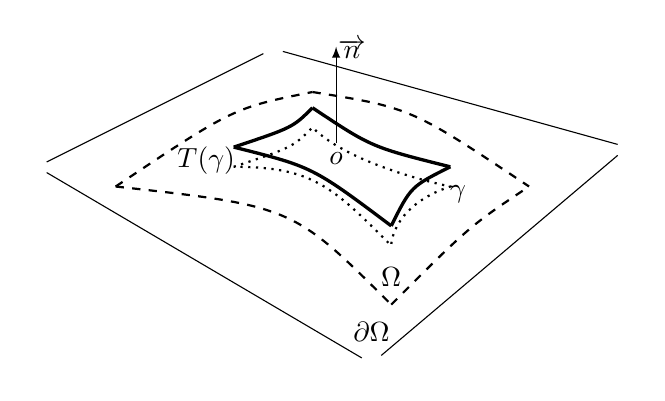
\begin{tikzpicture}[scale = 0.5]
\draw[dashed,thick] (-7.5,-1.5).. controls (-3,-2) and (-3,-2) .. (-0.5,-4.5);
\draw[dashed,thick](-0.5,-4.5) .. controls (1.5,-2.5) and (1.5,-2.5) .. (3,-1.5);
\draw[dashed,thick] (-7.5,-1.5) .. controls (-4.5,0.5) and (-4.5,0.5) .. (-2.5,0.9);
\draw[dashed,thick] (-2.5,0.9) .. controls (0,0.5) and (0,0.5) .. (3,-1.5);
\node (v1) at (-3.5,2) {};
\node (v4) at (-9.5,-1) {};
\node (v3) at (-1,-6) {};
\node (v2) at (5.5,-0.5) {};
\draw  (v1) edge (v2);
\draw  (v2) edge (v3);
\draw  (v3) edge (v4);
\draw  (v4) edge (v1);
\draw [dotted,thick](-4.5,-1) .. controls (-3,-0.5) and (-3,-0.5) .. (-2.5,0) .. controls (-1.5,-1) and (1,-1.5) .. (1,-1.5) .. controls (-0.5,-2) and (-0.5,-3) .. (-0.5,-3) .. controls (-2,-1.5) and (-2.5,-1) .. (-4.5,-1);
\node at (-2,-1) {};
\node (v5) at (-1.9,-0.8) {$o$};
%\draw[] at (-2,-1) ;
\draw[very thick] (-4.5,-0.5) .. controls (-2.5,-1) and (-2.5,-1) .. (-0.5,-2.5) ;
\draw[very thick]  (-0.5,-2.5) .. controls (0,-1.5) and (0,-1.5) .. (1,-1);
\draw [very thick] (1,-1) .. controls (-1,-0.5) and (-1,-0.5) .. (-2.5,0.5);
\draw  [very thick](-2.5,0.5) .. controls (-3,0) and (-3,0) .. (-4.5,-0.5);
\node at (-0.5,-3.8) {$\Omega$};
\node at (-1,-5.2) {$\partial \Omega$};
\node at (1.2,-1.7) {$ \gamma$};
\node at (-5.2,-0.83) {$ T(\gamma)$};
\node at (-2,-1) {};
\node (v6) at (-1.9,2.3) {};
\draw[-latex]  (v5) edge (v6);
\node at (-1.5,2) {$\overrightarrow{n}$};
\end{tikzpicture}}
	\qquad
    \subfloat[]{            
\tikzmath{\dR=1.9;\da=-10.0;\dT=-0.59;\dD=-27.; \dV=-9.00;
\ra=7.5; \rb = \ra+\dR;
\rc=10.4; \rd = \rc+\dR;
\re=15.2; \rf = \re+0.1*\dR;
\rg=9.5; \rh = \rg+\dR;
\LNwee=0.5;
\LTree=1.3;
}

\begin{tikzpicture}[angle/.style={black,thick},]
\tdplotsetmaincoords{0}{10};
\pgfplotsset{every axis/.append style={
		%view={-30*(0*1)}{-30*(-3)},
		%view={-90}{-30*0},
		scale=1.1,
		axis lines=center,
		%axis on top,
		%xlabel={$y$},
		%ylabel={$x$},
		%zlabel={$z$},
               %axis x line=middle,    % put the x axis in the middle
               %axis y line=middle,    % put the y axis in the middle
                %axis z line=middle,    % put the z axis in the middle
               %axis line style={-stealth}, % arrows on the axis
               axis line style={draw=none},
               axis equal image,
,
            }}
    \pgfplotsset{ticks=none};
    \pgfplotsset{compat=1.12};
	\begin{axis}[]
			
		%*******************************    first geodesics  ***********************************
		\addplot [dashed,thin,decoration={markings, mark = at position 0.5 with {\arrow[scale = 2.5]{latex[reversed]}}},postaction ={decorate},samples=40,	samples y=0,	domain=90.0+10:0-10]
		({-4.5+\ra*cos(x)},{-4.5+\ra*sin(x)})node[above,left] {$\gamma_{1}$};
		
		
      		\def \f{19.6}%********************************************
      		\def\fe{-2}
	
      		\def \fff{77.2}%********************************************
	
  		%second geodesics **************************************
  			
		\addplot [dashed,thin,decoration={markings, mark = at position 0.6 with  {\arrow[scale = 2.5]{latex[reversed]}}},postaction ={decorate},samples=40,	samples y=0,	domain=300+80:295]({-9.1+\rg*cos(x)},{10+\rg*sin(x)})node[below,left,{anchor=north west}] {$\gamma_{2}$};
		
		\def\qt{2.55};
	
      		
      		
  		\def\mbt{-49};
  		
 		%***************************                           third geodesics                 *********************************
 		
		\addplot [dashed,thin,decoration={markings, mark = at position 0.5 with {\arrow[scale = 2.5]{latex[reversed]}}},postaction ={decorate},samples=40,	samples y=0,	domain=0-35:70.0+45]({\rc*cos(x)},{\rc*sin(x)})node[below,left] {$\gamma_{3}$};
		
		\def\w{-15};
	
  		\def\ww{88};
			
  		%************************************************ fourth geodesics **************************************
  				
		\addplot [dashed,thin,decoration={markings, mark = at position 0.5 with {\arrow[scale = 2.5]{latex[reversed]}}},postaction ={decorate},samples=40,	samples y=0,	domain=270.0+20:270.0-30]({5-\re*cos(x)},{-17-\re*sin(x)})node[below,left] {$ \gamma_{4} \ $};
		
		\def\q{109.5};
 		
  		\def\mb{81};
		
    
%********************* angles between the 4 geodesic paths
				% ***************************** 1 and 4 *************************
					
	  	\draw[-Latex,black,  thin] let
   		 \p0 = ({-4.5+\ra*cos(\f)},{-4.5+\ra*sin(\f)}),
    		\p1 =   ({5+\re*cos(\mb+\dV)},{-17+1.1*\re*sin(\mb+\dV)}) ,
    		\p2 =  ({-4.5+\ra*cos(\f-\da)},{-4.5+\ra*sin(\f-\da)}),
    		\n1 = {atan2(\y1 - \y0,\x1 - \x0)},
    		\n2 = {atan2(\y2 - \y0,\x2 - \x0)},
    		\n3 = {0.6cm},
    		\n4 = {(\n1 + \n2) / 2}
  		in ({-4.5+\ra*cos(\f)},{-4.5+\ra*sin(\f)}) +(\n1:\n3) arc[radius = \n3, start angle = \n1, end angle = \n2]node[midway,{anchor=south}] {$\ \ \Psi_{4\rightarrow 1}$};;
				
				% ***************************** 1 and 2 *************************
					
	  	\draw[-Latex,,black,  thin] let
   		\p0 = ({-4.5+\ra*cos(\fff)},{-4.5+\ra*sin(\fff)}),
    		\p1 =   ( {-4.5+\ra*cos(\fff+\da)},{-4.5+\ra*sin(\fff+\da)}),
    		\p2 =({-9.1+\rg*cos(\mbt-\dD)},{10+1.19*\rg*sin(\mbt-\dD)}),
    		\n1 = {atan2(\y1 - \y0,\x1 - \x0)},
    		\n2 = {atan2(\y2 - \y0,\x2 - \x0)},
    		\n3 = {0.65cm},
    		\n4 = {(\n1 + \n2) / 2}
  		in ({-4.5+\ra*cos(\fff)},{-4.5+\ra*sin(\fff)}) +(\n1:\n3) arc[radius = \n3, start angle = \n1, end angle = \n2]node[midway,right]{$\Psi_{1\rightarrow 2}$};		
				
				% ***************************** 2 and 3  *************************
		 \draw[-Latex,black,  thin] let
   		 \p0 = ({\rc*cos(\ww)},{\rc*sin(\ww)}),
    		\p1 =   ({-9.1+1.1*\rg*cos(\qt+\dD)},{10+1.1*\rg*sin(\qt+\dD)}) ,
    		\p2 =  ({\rc*cos(\ww+\dT)},{\rc*sin(\ww+\dT)}),
    		\n1 = {atan2(\y1 - \y0,\x1 - \x0)},
    		\n2 = {atan2(\y2 - \y0,\x2 - \x0)},
    		\n3 = {0.8cm},
    		\n4 = {(\n1 + \n2) / 2}
  		in ({\rc*cos(\ww)},{\rc*sin(\ww)}) +(\n1:\n3) arc[radius = \n3, start angle = \n1, end angle = \n2]node[midway,right ] {$\  \ \Psi_{2\rightarrow 3}$};	
			
			
						% ***************************** 3 and 4  *************************
		 \draw[-Latex,black,  thin] let
   		 \p0 = ({\rc*cos(\w)},{\rc*sin(\w)},0),
    		\p1 =  ({\rc*cos(\w+\dT)},{1.04*\rc*sin(\w+\dT)}),
    		\p2 =({5-\rf*cos(\q-\dV)},{-17+\rf*sin(\q-\dV)}),
    		\n1 = {atan2(\y1 - \y0,\x1 - \x0)},
    		\n2 = {atan2(\y2 - \y0,\x2 - \x0)},
    		\n3 = {-0.8cm},
    		\n4 = {(\n1 + \n2) / 2}
  		in ({\rc*cos(\w)},{\rc*sin(\w)}) +(\n1:\n3) arc[radius = \n3, start angle = \n1, end angle = \n2]node[midway,{anchor=south}] {$ \Psi_{3\rightarrow 4} \ \ \ \ \ $};	
		\draw[very  thick]({\rc*cos(\w)},{\rc*sin(\w)},)-- ({\rc*cos(\ww)},{\rc*sin(\ww)});
		\draw[very  thick]({-4.5+\ra*cos(\fff)},{-4.5+\ra*sin(\fff)})-- ({\rc*cos(\ww)},{\rc*sin(\ww)});
		\draw[very  thick]({-4.5+\ra*cos(\fff)},{-4.5+\ra*sin(\fff)})-- ({-4.5+\ra*cos(\f)},{-4.5+\ra*sin(\f)});
		\draw[very thick]({\rc*cos(\w)},{\rc*sin(\w)})-- ({-4.5+\ra*cos(\f)},{-4.5+\ra*sin(\f)});
		
		\def \fet{-0.27};
 		\draw[thick, -Latex]({-9.1+\rg*cos(\mbt)},{10+\rg*sin(\mbt)}) -- ({(1-\fet)*(-9.1+\rg*cos(\mbt))+\fet*(-9.1+\rg*cos(\mbt+\dD))},{(1-\fet)*(10+\rg*sin(\mbt))+\fet*(10+1.2*\rg*sin(\mbt+\dD))})node[below,right] {};
 		\def\fe{1}
 		 \draw[thick, -Latex]({-4.5+\ra*cos(\fff)},{-4.5+\ra*sin(\fff)},0) -- ({(1-\fe)*(-4.5+\ra*cos(\fff))+\fe*(-4.5+\ra*cos(\fff+\da))},{(1-\fe)*(-4.5+\ra*sin(\fff))+\fe*(-4.5+\ra*sin(\fff+\da))},0)node[{anchor=south west}]  {};		
  		  
		  \node[{anchor=north east}]  at ({-4.5+\ra*cos(\f)},{-4.5+\ra*sin(\f)}){$p_1$};
		 \node[{anchor=south east}]  at ({-4.5+\ra*cos(\fff)},{-4.5+\ra*sin(\fff)}){$p_2$};
		  \node[{anchor=south east}]  at ({\rc*cos(\ww)},{\rc*sin(\ww)}){$p_3$};
		   \node[{anchor=south west}]  at ({\rc*cos(\w)},{\rc*sin(\w)}){$p_4$};
  		 \draw[Latex-,black,  thin] let
   		 \p0 = ({-4.5+\ra*cos(\fff)},{-4.5+\ra*sin(\fff)}),
    		\p1 =   ({\rc*cos(\ww)},{\rc*sin(\ww)}),
    		\p2 =({-4.5+\ra*cos(\f)},{-4.5+\ra*sin(\f)}),
    		\n1 = {atan2(\y1 - \y0,\x1 - \x0)},
    		\n2 = {atan2(\y2 - \y0,\x2 - \x0)},
    		\n3 = {1.7cm},
    		\n4 = {(\n1 + \n2) / 2}
  		in({-4.5+\ra*cos(\fff)},{-4.5+\ra*sin(\fff)}) +(\n1:\n3) arc[radius = \n3, start angle = \n1, end angle = \n2]node[midway,right ] {$\nu_{2}$};	
		
  		
  		
\end{axis}
\end{tikzpicture}}
\caption{Relationship between parallel transportation along a closed path and the excess of the angle-sum over four right angles of a quadrilateral.}
\end{figure}

$$\blacklozenge$$
\newpage